% Options for packages loaded elsewhere
\PassOptionsToPackage{unicode}{hyperref}
\PassOptionsToPackage{hyphens}{url}
%
\documentclass[
]{book}
\usepackage{amsmath,amssymb}
\usepackage{lmodern}
\usepackage{ifxetex,ifluatex}
\ifnum 0\ifxetex 1\fi\ifluatex 1\fi=0 % if pdftex
  \usepackage[T1]{fontenc}
  \usepackage[utf8]{inputenc}
  \usepackage{textcomp} % provide euro and other symbols
\else % if luatex or xetex
  \usepackage{unicode-math}
  \defaultfontfeatures{Scale=MatchLowercase}
  \defaultfontfeatures[\rmfamily]{Ligatures=TeX,Scale=1}
\fi
% Use upquote if available, for straight quotes in verbatim environments
\IfFileExists{upquote.sty}{\usepackage{upquote}}{}
\IfFileExists{microtype.sty}{% use microtype if available
  \usepackage[]{microtype}
  \UseMicrotypeSet[protrusion]{basicmath} % disable protrusion for tt fonts
}{}
\makeatletter
\@ifundefined{KOMAClassName}{% if non-KOMA class
  \IfFileExists{parskip.sty}{%
    \usepackage{parskip}
  }{% else
    \setlength{\parindent}{0pt}
    \setlength{\parskip}{6pt plus 2pt minus 1pt}}
}{% if KOMA class
  \KOMAoptions{parskip=half}}
\makeatother
\usepackage{xcolor}
\IfFileExists{xurl.sty}{\usepackage{xurl}}{} % add URL line breaks if available
\IfFileExists{bookmark.sty}{\usepackage{bookmark}}{\usepackage{hyperref}}
\hypersetup{
  pdftitle={STAT 454 Bayesian Statistics: Short term COVID-19 prediction model using MCMC simulation},
  pdfauthor={Raymond Gu, Zefan Qian},
  hidelinks,
  pdfcreator={LaTeX via pandoc}}
\urlstyle{same} % disable monospaced font for URLs
\usepackage{color}
\usepackage{fancyvrb}
\newcommand{\VerbBar}{|}
\newcommand{\VERB}{\Verb[commandchars=\\\{\}]}
\DefineVerbatimEnvironment{Highlighting}{Verbatim}{commandchars=\\\{\}}
% Add ',fontsize=\small' for more characters per line
\usepackage{framed}
\definecolor{shadecolor}{RGB}{248,248,248}
\newenvironment{Shaded}{\begin{snugshade}}{\end{snugshade}}
\newcommand{\AlertTok}[1]{\textcolor[rgb]{0.94,0.16,0.16}{#1}}
\newcommand{\AnnotationTok}[1]{\textcolor[rgb]{0.56,0.35,0.01}{\textbf{\textit{#1}}}}
\newcommand{\AttributeTok}[1]{\textcolor[rgb]{0.77,0.63,0.00}{#1}}
\newcommand{\BaseNTok}[1]{\textcolor[rgb]{0.00,0.00,0.81}{#1}}
\newcommand{\BuiltInTok}[1]{#1}
\newcommand{\CharTok}[1]{\textcolor[rgb]{0.31,0.60,0.02}{#1}}
\newcommand{\CommentTok}[1]{\textcolor[rgb]{0.56,0.35,0.01}{\textit{#1}}}
\newcommand{\CommentVarTok}[1]{\textcolor[rgb]{0.56,0.35,0.01}{\textbf{\textit{#1}}}}
\newcommand{\ConstantTok}[1]{\textcolor[rgb]{0.00,0.00,0.00}{#1}}
\newcommand{\ControlFlowTok}[1]{\textcolor[rgb]{0.13,0.29,0.53}{\textbf{#1}}}
\newcommand{\DataTypeTok}[1]{\textcolor[rgb]{0.13,0.29,0.53}{#1}}
\newcommand{\DecValTok}[1]{\textcolor[rgb]{0.00,0.00,0.81}{#1}}
\newcommand{\DocumentationTok}[1]{\textcolor[rgb]{0.56,0.35,0.01}{\textbf{\textit{#1}}}}
\newcommand{\ErrorTok}[1]{\textcolor[rgb]{0.64,0.00,0.00}{\textbf{#1}}}
\newcommand{\ExtensionTok}[1]{#1}
\newcommand{\FloatTok}[1]{\textcolor[rgb]{0.00,0.00,0.81}{#1}}
\newcommand{\FunctionTok}[1]{\textcolor[rgb]{0.00,0.00,0.00}{#1}}
\newcommand{\ImportTok}[1]{#1}
\newcommand{\InformationTok}[1]{\textcolor[rgb]{0.56,0.35,0.01}{\textbf{\textit{#1}}}}
\newcommand{\KeywordTok}[1]{\textcolor[rgb]{0.13,0.29,0.53}{\textbf{#1}}}
\newcommand{\NormalTok}[1]{#1}
\newcommand{\OperatorTok}[1]{\textcolor[rgb]{0.81,0.36,0.00}{\textbf{#1}}}
\newcommand{\OtherTok}[1]{\textcolor[rgb]{0.56,0.35,0.01}{#1}}
\newcommand{\PreprocessorTok}[1]{\textcolor[rgb]{0.56,0.35,0.01}{\textit{#1}}}
\newcommand{\RegionMarkerTok}[1]{#1}
\newcommand{\SpecialCharTok}[1]{\textcolor[rgb]{0.00,0.00,0.00}{#1}}
\newcommand{\SpecialStringTok}[1]{\textcolor[rgb]{0.31,0.60,0.02}{#1}}
\newcommand{\StringTok}[1]{\textcolor[rgb]{0.31,0.60,0.02}{#1}}
\newcommand{\VariableTok}[1]{\textcolor[rgb]{0.00,0.00,0.00}{#1}}
\newcommand{\VerbatimStringTok}[1]{\textcolor[rgb]{0.31,0.60,0.02}{#1}}
\newcommand{\WarningTok}[1]{\textcolor[rgb]{0.56,0.35,0.01}{\textbf{\textit{#1}}}}
\usepackage{longtable,booktabs,array}
\usepackage{calc} % for calculating minipage widths
% Correct order of tables after \paragraph or \subparagraph
\usepackage{etoolbox}
\makeatletter
\patchcmd\longtable{\par}{\if@noskipsec\mbox{}\fi\par}{}{}
\makeatother
% Allow footnotes in longtable head/foot
\IfFileExists{footnotehyper.sty}{\usepackage{footnotehyper}}{\usepackage{footnote}}
\makesavenoteenv{longtable}
\usepackage{graphicx}
\makeatletter
\def\maxwidth{\ifdim\Gin@nat@width>\linewidth\linewidth\else\Gin@nat@width\fi}
\def\maxheight{\ifdim\Gin@nat@height>\textheight\textheight\else\Gin@nat@height\fi}
\makeatother
% Scale images if necessary, so that they will not overflow the page
% margins by default, and it is still possible to overwrite the defaults
% using explicit options in \includegraphics[width, height, ...]{}
\setkeys{Gin}{width=\maxwidth,height=\maxheight,keepaspectratio}
% Set default figure placement to htbp
\makeatletter
\def\fps@figure{htbp}
\makeatother
\setlength{\emergencystretch}{3em} % prevent overfull lines
\providecommand{\tightlist}{%
  \setlength{\itemsep}{0pt}\setlength{\parskip}{0pt}}
\setcounter{secnumdepth}{5}
\usepackage{booktabs}
\usepackage{amsthm}
\makeatletter
\def\thm@space@setup{%
  \thm@preskip=8pt plus 2pt minus 4pt
  \thm@postskip=\thm@preskip
}
\makeatother
\ifluatex
  \usepackage{selnolig}  % disable illegal ligatures
\fi
\usepackage[]{natbib}
\bibliographystyle{apalike}

\title{STAT 454 Bayesian Statistics: Short term COVID-19 prediction model using MCMC simulation}
\author{Raymond Gu, Zefan Qian}
\date{2021-12-13}

\begin{document}
\maketitle

{
\setcounter{tocdepth}{1}
\tableofcontents
}
\hypertarget{preface}{%
\chapter{Preface}\label{preface}}

This is the bookdown of Raymond and Zefan's STAT 454 Bayesian Statistics Project.

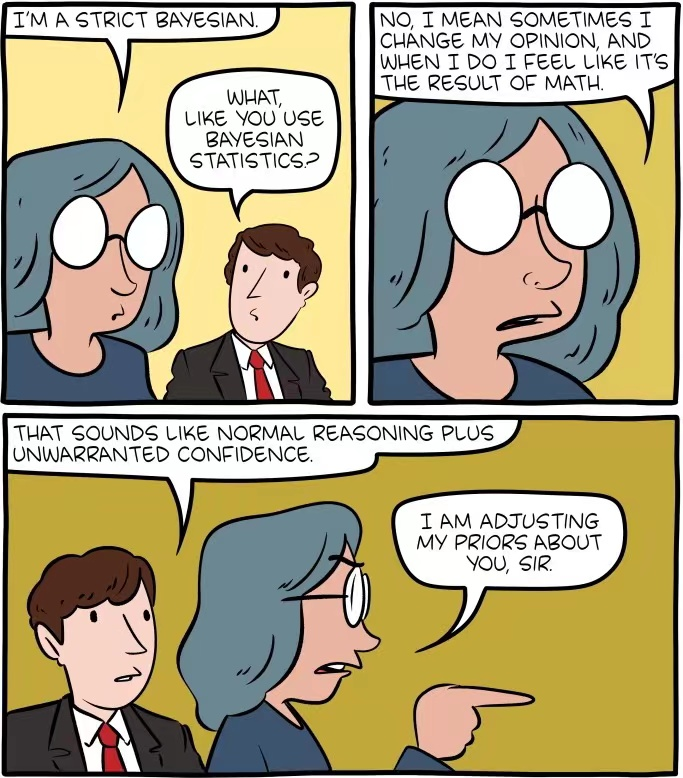
\includegraphics{preface_comic.jpg}

Credit to \href{smbc-comics.com}{SMBC}.

\hypertarget{intro}{%
\chapter{Motivation}\label{intro}}

First identified in Botswana and South Africa, this new iteration of the coronavirus Omicron has prompted concern among scientists and public health officials because of an unusually high number of mutations that have the potential to make the virus more transmissible and less susceptible to existing vaccines. Hence a big question for humanity is: when will it end or at least not affect people's lives? In our report, we aim to investigate how factors such as state and time can help us predict future outbreaks. The investigation potentially can help people decide to what places and at what time are they safe to travel if they have to.

\hypertarget{data}{%
\chapter{Data}\label{data}}

\hypertarget{data-source}{%
\section{Data Source}\label{data-source}}

Our data was collected from the New York Times, which is an American daily newspaper based in New York City with a worldwide readership. The data is held on New York Times COVID-19 Github repository. This data includes cumulative cases and deaths reported in each state across the U.S., including U.S. territories and the District of Columbia, since the beginning of the pandemic beginning in Jan 21, 2021. The data is still updating, so we ignore Dec 2021 data and use all the data until Nov 30, 2021.

Website for our data source: \url{https://raw.githubusercontent.com/nytimes/covid-19-data/master/us-states.csv}

\hypertarget{data-dictionary}{%
\section{Data Dictionary}\label{data-dictionary}}

\begin{longtable}[]{@{}ll@{}}
\toprule
Variable Name & Description \\
\midrule
\endhead
date & Date \\
state & Name of State \\
fips & First Two Digits of ZipCode of the State \\
cases & Number of Cumulative Cases \\
deaths & Number of Cumulative Deaths \\
\bottomrule
\end{longtable}

\hypertarget{data-cleaning}{%
\chapter{Data Cleaning}\label{data-cleaning}}

\begin{Shaded}
\begin{Highlighting}[]
\CommentTok{\#load packages}
\FunctionTok{library}\NormalTok{(bayesrules)}
\FunctionTok{library}\NormalTok{(tidyverse)}
\FunctionTok{library}\NormalTok{(janitor)}
\FunctionTok{library}\NormalTok{(rstanarm)}
\FunctionTok{library}\NormalTok{(bayesplot)}
\FunctionTok{library}\NormalTok{(tidybayes)}
\FunctionTok{library}\NormalTok{(broom.mixed)}
\FunctionTok{library}\NormalTok{(modelr)}
\FunctionTok{library}\NormalTok{(e1071)}
\FunctionTok{library}\NormalTok{(forcats)}
\FunctionTok{library}\NormalTok{(ggExtra)}
\FunctionTok{library}\NormalTok{(ggpubr)}
\FunctionTok{library}\NormalTok{(ggridges)}
\FunctionTok{library}\NormalTok{(devtools)}
\FunctionTok{library}\NormalTok{(zoo)}
\FunctionTok{library}\NormalTok{(DT)}
\FunctionTok{library}\NormalTok{(dplyr)}
\FunctionTok{library}\NormalTok{(plyr)}
\FunctionTok{Sys.setlocale}\NormalTok{(}\StringTok{"LC\_TIME"}\NormalTok{, }\StringTok{"English"}\NormalTok{)}
\end{Highlighting}
\end{Shaded}

\begin{verbatim}
## [1] "English_United States.1252"
\end{verbatim}

\hypertarget{load-data}{%
\section{Load Data}\label{load-data}}

\begin{Shaded}
\begin{Highlighting}[]
\CommentTok{\#load data}
\NormalTok{covid19 }\OtherTok{\textless{}{-}} \FunctionTok{read\_csv}\NormalTok{(}\FunctionTok{url}\NormalTok{(}\StringTok{"https://raw.githubusercontent.com/nytimes/covid{-}19{-}data/master/us{-}states.csv"}\NormalTok{))}
\end{Highlighting}
\end{Shaded}

\hypertarget{generate-monthly-incident-data}{%
\section{Generate Monthly Incident Data}\label{generate-monthly-incident-data}}

Here, we generate the daily incident data by subtracting the lagging of yesterday from the cumulative number of COVID-19 cases at present. By summing all daily incident data within one month, we generate the monthly incident data.

\begin{Shaded}
\begin{Highlighting}[]
\NormalTok{covid19\_filter }\OtherTok{\textless{}{-}}\NormalTok{ covid19 }\SpecialCharTok{\%\textgreater{}\%}
\NormalTok{  dplyr}\SpecialCharTok{::}\FunctionTok{group\_by}\NormalTok{(state) }\SpecialCharTok{\%\textgreater{}\%}
\NormalTok{  dplyr}\SpecialCharTok{::}\FunctionTok{mutate}\NormalTok{(}\AttributeTok{lag1 =} \FunctionTok{lag}\NormalTok{(cases, }\AttributeTok{n =} \DecValTok{1}\NormalTok{)) }

\NormalTok{covid19\_filter }\OtherTok{\textless{}{-}}\NormalTok{ covid19\_filter }\SpecialCharTok{\%\textgreater{}\%}
  \FunctionTok{mutate}\NormalTok{(}\AttributeTok{lag1 =}\NormalTok{ lag1 }\SpecialCharTok{\%\textgreater{}\%} 
           \FunctionTok{replace\_na}\NormalTok{(}\DecValTok{0}\NormalTok{))}

\NormalTok{covid19\_filter }\OtherTok{\textless{}{-}}\NormalTok{ covid19\_filter }\SpecialCharTok{\%\textgreater{}\%} \FunctionTok{mutate}\NormalTok{(}\AttributeTok{case\_new =}\NormalTok{ cases }\SpecialCharTok{{-}}\NormalTok{ lag1) }
\end{Highlighting}
\end{Shaded}

\hypertarget{generate-time-variables}{%
\section{Generate Time Variables}\label{generate-time-variables}}

\begin{Shaded}
\begin{Highlighting}[]
\NormalTok{covid19\_month }\OtherTok{\textless{}{-}}\NormalTok{ covid19\_filter }\SpecialCharTok{\%\textgreater{}\%}
\NormalTok{  dplyr}\SpecialCharTok{::}\FunctionTok{mutate}\NormalTok{(}\AttributeTok{year =}\NormalTok{ lubridate}\SpecialCharTok{::}\FunctionTok{year}\NormalTok{(date), }
                \AttributeTok{month =}\NormalTok{ lubridate}\SpecialCharTok{::}\FunctionTok{month}\NormalTok{(date), }
                \AttributeTok{day =}\NormalTok{ lubridate}\SpecialCharTok{::}\FunctionTok{day}\NormalTok{(date)) }\SpecialCharTok{\%\textgreater{}\%}
\NormalTok{  dplyr}\SpecialCharTok{::}\FunctionTok{group\_by}\NormalTok{(state, year, month) }\SpecialCharTok{\%\textgreater{}\%}
\NormalTok{  dplyr}\SpecialCharTok{::}\FunctionTok{summarize}\NormalTok{(}\AttributeTok{cases =} \FunctionTok{sum}\NormalTok{(case\_new)) }

\NormalTok{covid19\_month }\OtherTok{\textless{}{-}}\NormalTok{ covid19\_month }\SpecialCharTok{\%\textgreater{}\%}
  \FunctionTok{mutate}\NormalTok{(}\AttributeTok{Date =} \FunctionTok{as.yearmon}\NormalTok{(}\FunctionTok{paste}\NormalTok{(covid19\_month}\SpecialCharTok{$}\NormalTok{year, covid19\_month}\SpecialCharTok{$}\NormalTok{month), }\StringTok{"\%Y \%m"}\NormalTok{))}
\end{Highlighting}
\end{Shaded}

\hypertarget{remove-incomplete-monthly-data}{%
\section{Remove Incomplete Monthly Data}\label{remove-incomplete-monthly-data}}

Since before the time we submit this project, we do not have complete data for December, 2021, we decide to remove the incomplete data from our dataset.

\begin{Shaded}
\begin{Highlighting}[]
\NormalTok{covid19\_month }\OtherTok{\textless{}{-}}\NormalTok{ covid19\_month }\SpecialCharTok{\%\textgreater{}\%}
  \FunctionTok{filter}\NormalTok{(}\SpecialCharTok{!}\NormalTok{(year }\SpecialCharTok{==} \DecValTok{2021} \SpecialCharTok{\&}\NormalTok{ month }\SpecialCharTok{==} \DecValTok{12}\NormalTok{)) }
\end{Highlighting}
\end{Shaded}

\hypertarget{generate-daily-average-number-of-cases-within-one-month}{%
\section{Generate Daily Average Number of Cases within One Month}\label{generate-daily-average-number-of-cases-within-one-month}}

We take the daily average of the number of COVID-19 cases that appear within one month because different months have different days. We would like to minimize the impacts from this difference.

\begin{Shaded}
\begin{Highlighting}[]
\NormalTok{covid19\_month }\OtherTok{\textless{}{-}}\NormalTok{ covid19\_month }\SpecialCharTok{\%\textgreater{}\%}
  \FunctionTok{mutate}\NormalTok{(}\AttributeTok{cases\_daily =} \FunctionTok{round}\NormalTok{(}\FunctionTok{ifelse}\NormalTok{(month }\SpecialCharTok{==} \DecValTok{1} \SpecialCharTok{|}\NormalTok{ month }\SpecialCharTok{==} \DecValTok{3} \SpecialCharTok{|}\NormalTok{ month }\SpecialCharTok{==} \DecValTok{5} \SpecialCharTok{|}\NormalTok{ month }\SpecialCharTok{==} \DecValTok{7} \SpecialCharTok{|}\NormalTok{ month }\SpecialCharTok{==} \DecValTok{8} \SpecialCharTok{|}\NormalTok{ month }\SpecialCharTok{==} \DecValTok{10} \SpecialCharTok{|}\NormalTok{ month }\SpecialCharTok{==} \DecValTok{12}\NormalTok{, cases }\SpecialCharTok{/} \DecValTok{31}\NormalTok{, }\FunctionTok{ifelse}\NormalTok{(month }\SpecialCharTok{==} \DecValTok{4} \SpecialCharTok{|}\NormalTok{ month }\SpecialCharTok{==} \DecValTok{6} \SpecialCharTok{|}\NormalTok{ month }\SpecialCharTok{==} \DecValTok{9} \SpecialCharTok{|}\NormalTok{ month }\SpecialCharTok{==} \DecValTok{11}\NormalTok{, cases}\SpecialCharTok{/} \DecValTok{30}\NormalTok{, }\FunctionTok{ifelse}\NormalTok{(month }\SpecialCharTok{==} \DecValTok{2} \SpecialCharTok{\&}\NormalTok{ year }\SpecialCharTok{==} \DecValTok{2020}\NormalTok{, cases }\SpecialCharTok{/} \DecValTok{29}\NormalTok{, cases }\SpecialCharTok{/}\DecValTok{28}\NormalTok{)))))}
\end{Highlighting}
\end{Shaded}

\hypertarget{generate-lag-in-time-series}{%
\section{Generate Lag in Time-Series}\label{generate-lag-in-time-series}}

\begin{Shaded}
\begin{Highlighting}[]
\NormalTok{covid19\_month }\OtherTok{\textless{}{-}}\NormalTok{ covid19\_month }\SpecialCharTok{\%\textgreater{}\%}
\NormalTok{  dplyr}\SpecialCharTok{::}\FunctionTok{group\_by}\NormalTok{(state) }\SpecialCharTok{\%\textgreater{}\%}
  \FunctionTok{mutate}\NormalTok{(}\AttributeTok{lag1 =} \FunctionTok{lag}\NormalTok{(cases\_daily, }\AttributeTok{n =} \DecValTok{1}\NormalTok{)) }\SpecialCharTok{\%\textgreater{}\%}
  \FunctionTok{mutate}\NormalTok{(}\AttributeTok{lag3 =} \FunctionTok{lag}\NormalTok{(cases\_daily, }\AttributeTok{n =} \DecValTok{3}\NormalTok{)) }\SpecialCharTok{\%\textgreater{}\%}
  \FunctionTok{mutate}\NormalTok{(}\AttributeTok{lag6 =} \FunctionTok{lag}\NormalTok{(cases\_daily, }\AttributeTok{n =} \DecValTok{6}\NormalTok{)) }

\NormalTok{covid19\_month }\OtherTok{\textless{}{-}}\NormalTok{ covid19\_month }\SpecialCharTok{\%\textgreater{}\%} 
  \FunctionTok{mutate}\NormalTok{(}\AttributeTok{lag1 =}\NormalTok{ lag1 }\SpecialCharTok{\%\textgreater{}\%} \FunctionTok{replace\_na}\NormalTok{(}\DecValTok{0}\NormalTok{)) }\SpecialCharTok{\%\textgreater{}\%}
  \FunctionTok{mutate}\NormalTok{(}\AttributeTok{lag3 =}\NormalTok{ lag3 }\SpecialCharTok{\%\textgreater{}\%} \FunctionTok{replace\_na}\NormalTok{(}\DecValTok{0}\NormalTok{)) }\SpecialCharTok{\%\textgreater{}\%}
  \FunctionTok{mutate}\NormalTok{(}\AttributeTok{lag6 =}\NormalTok{ lag6 }\SpecialCharTok{\%\textgreater{}\%} \FunctionTok{replace\_na}\NormalTok{(}\DecValTok{0}\NormalTok{))}
\end{Highlighting}
\end{Shaded}

\hypertarget{clean-undefined-values-0-in-logarithmic-function}{%
\section{Clean undefined values (0) in Logarithmic function}\label{clean-undefined-values-0-in-logarithmic-function}}

Since log(0) is undefined, we remove 0 from our dataset by adding one to the lagging variables.

\begin{Shaded}
\begin{Highlighting}[]
\NormalTok{covid19\_month }\OtherTok{\textless{}{-}}\NormalTok{ covid19\_month }\SpecialCharTok{\%\textgreater{}\%}
  \FunctionTok{mutate}\NormalTok{(}\AttributeTok{lag1 =}\NormalTok{ lag1 }\SpecialCharTok{+} \DecValTok{1}\NormalTok{) }\SpecialCharTok{\%\textgreater{}\%}
  \FunctionTok{mutate}\NormalTok{(}\AttributeTok{lag3 =}\NormalTok{ lag3 }\SpecialCharTok{+} \DecValTok{1}\NormalTok{) }\SpecialCharTok{\%\textgreater{}\%}
  \FunctionTok{mutate}\NormalTok{(}\AttributeTok{lag6 =}\NormalTok{ lag6 }\SpecialCharTok{+} \DecValTok{1}\NormalTok{)}

\NormalTok{covid19\_month }\OtherTok{\textless{}{-}}\NormalTok{ covid19\_month }\SpecialCharTok{\%\textgreater{}\%}
  \FunctionTok{mutate}\NormalTok{(}\AttributeTok{lag1\_log =} \FunctionTok{log}\NormalTok{(lag1)) }\SpecialCharTok{\%\textgreater{}\%}
  \FunctionTok{mutate}\NormalTok{(}\AttributeTok{lag3\_log =} \FunctionTok{log}\NormalTok{(lag3)) }\SpecialCharTok{\%\textgreater{}\%}
  \FunctionTok{mutate}\NormalTok{(}\AttributeTok{lag6\_log =} \FunctionTok{log}\NormalTok{(lag6))}
\end{Highlighting}
\end{Shaded}

\hypertarget{generate-season-variable}{%
\section{Generate Season Variable}\label{generate-season-variable}}

\begin{Shaded}
\begin{Highlighting}[]
\NormalTok{covid19\_month }\OtherTok{\textless{}{-}}\NormalTok{ covid19\_month }\SpecialCharTok{\%\textgreater{}\%}
  \FunctionTok{mutate}\NormalTok{(}\AttributeTok{season =} \FunctionTok{ifelse}\NormalTok{(month }\SpecialCharTok{\textgreater{}=} \DecValTok{3} \SpecialCharTok{\&}\NormalTok{ month }\SpecialCharTok{\textless{}=} \DecValTok{5}\NormalTok{ , }\StringTok{"spring"}\NormalTok{, }\FunctionTok{ifelse}\NormalTok{(month }\SpecialCharTok{\textgreater{}=} \DecValTok{6} \SpecialCharTok{\&}\NormalTok{ month }\SpecialCharTok{\textless{}=} \DecValTok{8}\NormalTok{, }\StringTok{"summer"}\NormalTok{, }\FunctionTok{ifelse}\NormalTok{(month }\SpecialCharTok{\textgreater{}=} \DecValTok{9} \SpecialCharTok{\&}\NormalTok{ month }\SpecialCharTok{\textless{}=} \DecValTok{11}\NormalTok{, }\StringTok{"fall"}\NormalTok{, }\StringTok{"winter"}\NormalTok{))))}
\end{Highlighting}
\end{Shaded}

\hypertarget{generate-indicator-variable-for-vaccination}{%
\section{Generate Indicator Variable for Vaccination}\label{generate-indicator-variable-for-vaccination}}

\begin{Shaded}
\begin{Highlighting}[]
\NormalTok{covid19\_month }\OtherTok{\textless{}{-}}\NormalTok{ covid19\_month }\SpecialCharTok{\%\textgreater{}\%}
  \FunctionTok{mutate}\NormalTok{(}\AttributeTok{vaccine =} \FunctionTok{ifelse}\NormalTok{(year }\SpecialCharTok{==} \DecValTok{2021} \SpecialCharTok{\&}\NormalTok{ month }\SpecialCharTok{\textgreater{}=} \DecValTok{3}\NormalTok{, }\DecValTok{1}\NormalTok{, }\DecValTok{0}\NormalTok{))}
\end{Highlighting}
\end{Shaded}

\hypertarget{generate-indicator-variable-for-appearance-of-delta-variant}{%
\section{Generate Indicator Variable for Appearance of Delta Variant}\label{generate-indicator-variable-for-appearance-of-delta-variant}}

\begin{Shaded}
\begin{Highlighting}[]
\NormalTok{covid19\_month }\OtherTok{\textless{}{-}}\NormalTok{ covid19\_month }\SpecialCharTok{\%\textgreater{}\%}
  \FunctionTok{mutate}\NormalTok{(}\AttributeTok{variant =} \FunctionTok{ifelse}\NormalTok{(year }\SpecialCharTok{==} \DecValTok{2021} \SpecialCharTok{\&}\NormalTok{ month }\SpecialCharTok{\textgreater{}=} \DecValTok{6}\NormalTok{, }\DecValTok{1}\NormalTok{, }\DecValTok{0}\NormalTok{))}
\end{Highlighting}
\end{Shaded}

\hypertarget{visualizations}{%
\chapter{Visualizations}\label{visualizations}}

In this chapter, we make visualizations to dig into what is our prior model and what factors can be used in our regression.

\hypertarget{general-trend-in-monthly-increases}{%
\section{General Trend in Monthly Increases}\label{general-trend-in-monthly-increases}}

First, let's see what the distribution of monthly case increases look like. The first three visualizations we have here are density plots that count the frequencies of monthly case increases, not relating to time or state. If we look at the United States as a whole, we see that the most frequent number of new cases in one month for the whole country is around 100,000.

\begin{Shaded}
\begin{Highlighting}[]
\NormalTok{covid19\_month }\SpecialCharTok{\%\textgreater{}\%}
  \FunctionTok{ggplot}\NormalTok{(}\FunctionTok{aes}\NormalTok{(}\AttributeTok{x =}\NormalTok{ cases)) }\SpecialCharTok{+}
  \FunctionTok{geom\_density}\NormalTok{() }\SpecialCharTok{+}
  \FunctionTok{labs}\NormalTok{(}\AttributeTok{x =} \StringTok{"Number of new cases in one month"}\NormalTok{, }\AttributeTok{y =} \StringTok{"Count"}\NormalTok{, }\AttributeTok{title =} \StringTok{"Distribution of number of new cases of US in one month"}\NormalTok{) }\SpecialCharTok{+}
  \FunctionTok{theme}\NormalTok{(}\AttributeTok{plot.title =} \FunctionTok{element\_text}\NormalTok{(}\AttributeTok{hjust =} \FloatTok{0.5}\NormalTok{))}
\end{Highlighting}
\end{Shaded}

\includegraphics{bookdown-demo_files/figure-latex/unnamed-chunk-12-1.pdf}

We can also look at individual state's distribution. The state of Minnesota and the state of California have similar distributions, but Minnesota has significantly fewer cases, probably due to less population.

\begin{Shaded}
\begin{Highlighting}[]
\NormalTok{covid19\_month }\SpecialCharTok{\%\textgreater{}\%}
  \FunctionTok{filter}\NormalTok{(state }\SpecialCharTok{==} \StringTok{"Minnesota"}\NormalTok{) }\SpecialCharTok{\%\textgreater{}\%}
  \FunctionTok{ggplot}\NormalTok{(}\FunctionTok{aes}\NormalTok{(}\AttributeTok{x =}\NormalTok{ cases)) }\SpecialCharTok{+}
  \FunctionTok{geom\_density}\NormalTok{() }\SpecialCharTok{+} 
  \FunctionTok{labs}\NormalTok{(}\AttributeTok{x =} \StringTok{"Number of new cases in one month"}\NormalTok{, }\AttributeTok{y =} \StringTok{"Count"}\NormalTok{, }\AttributeTok{title =} \StringTok{"Distribution of number of new cases of MN in one month"}\NormalTok{) }\SpecialCharTok{+}
  \FunctionTok{theme}\NormalTok{(}\AttributeTok{plot.title =} \FunctionTok{element\_text}\NormalTok{(}\AttributeTok{hjust =} \FloatTok{0.5}\NormalTok{))}
\end{Highlighting}
\end{Shaded}

\includegraphics{bookdown-demo_files/figure-latex/unnamed-chunk-13-1.pdf}

\begin{Shaded}
\begin{Highlighting}[]
\NormalTok{covid19\_month }\SpecialCharTok{\%\textgreater{}\%}
  \FunctionTok{filter}\NormalTok{(state }\SpecialCharTok{==} \StringTok{"California"}\NormalTok{) }\SpecialCharTok{\%\textgreater{}\%}
  \FunctionTok{ggplot}\NormalTok{(}\FunctionTok{aes}\NormalTok{(}\AttributeTok{x =}\NormalTok{ cases)) }\SpecialCharTok{+}
  \FunctionTok{geom\_density}\NormalTok{() }\SpecialCharTok{+}
  \FunctionTok{labs}\NormalTok{(}\AttributeTok{x =} \StringTok{"Number of new cases in one month"}\NormalTok{, }\AttributeTok{y =} \StringTok{"Count"}\NormalTok{, }\AttributeTok{title =} \StringTok{"Distribution of number of new cases of CA in one month"}\NormalTok{) }\SpecialCharTok{+}
  \FunctionTok{theme}\NormalTok{(}\AttributeTok{plot.title =} \FunctionTok{element\_text}\NormalTok{(}\AttributeTok{hjust =} \FloatTok{0.5}\NormalTok{))}
\end{Highlighting}
\end{Shaded}

\includegraphics{bookdown-demo_files/figure-latex/unnamed-chunk-14-1.pdf}

To relate these observations with our model choice, we will extend in the next Chapter.

\hypertarget{time-and-state}{%
\section{Time and State}\label{time-and-state}}

We are also able to show how the number of new cases for each month varies from state to state and time to time:

\textbf{For United States as the whole}

\begin{Shaded}
\begin{Highlighting}[]
\NormalTok{covid19\_month }\SpecialCharTok{\%\textgreater{}\%} 
\NormalTok{  dplyr}\SpecialCharTok{::}\FunctionTok{group\_by}\NormalTok{(Date) }\SpecialCharTok{\%\textgreater{}\%}
\NormalTok{  dplyr}\SpecialCharTok{::}\FunctionTok{summarize}\NormalTok{(}\AttributeTok{cases =} \FunctionTok{sum}\NormalTok{(cases)) }\SpecialCharTok{\%\textgreater{}\%}
  \FunctionTok{ggplot}\NormalTok{(}\FunctionTok{aes}\NormalTok{(}\AttributeTok{x =}\NormalTok{ Date, }\AttributeTok{y =}\NormalTok{ cases)) }\SpecialCharTok{+}
  \FunctionTok{geom\_line}\NormalTok{() }\SpecialCharTok{+} 
  \FunctionTok{geom\_vline}\NormalTok{(}\AttributeTok{xintercept =} \FloatTok{2021.167}\NormalTok{, }\AttributeTok{color =} \StringTok{"steelblue"}\NormalTok{) }\SpecialCharTok{+}
  \FunctionTok{geom\_vline}\NormalTok{(}\AttributeTok{xintercept =} \FloatTok{2021.450}\NormalTok{, }\AttributeTok{color =} \StringTok{"\#4f7c6e"}\NormalTok{) }\SpecialCharTok{+}
  \FunctionTok{labs}\NormalTok{(}\AttributeTok{x =} \StringTok{"Date"}\NormalTok{, }\AttributeTok{y =} \StringTok{"Number of new cases in each month"}\NormalTok{, }\AttributeTok{title =} \StringTok{"Number of new cases of US in one month changes over time"}\NormalTok{) }\SpecialCharTok{+}
  \FunctionTok{theme}\NormalTok{(}\AttributeTok{plot.title =} \FunctionTok{element\_text}\NormalTok{(}\AttributeTok{hjust =} \FloatTok{0.5}\NormalTok{))}
\end{Highlighting}
\end{Shaded}

\includegraphics{bookdown-demo_files/figure-latex/unnamed-chunk-15-1.pdf}

There are certain things that people are doing to prevent the virus including vaccines. Vaccines from Pfizer, Moderna, and Johnson \& Johnson, are being widely used starting March 2021, which is labeled as the line on the left in the graph. Some time later, we see a significant drop of monthly COVID-19 increases. However, the virus itself is quickly adapting as well. Around July, a variant called the Delta started to spread all over the world, more transmissible and less susceptible to existing vaccines, as indicated as the line on the right in the graph. As a result, the monthly case increases started to rise again. Because of how drastic the vaccines and virus variants can impact COVID infections, we would like to include these two as independent variables in our model. Specifically, they can only take on the value of 0 and 1. So it either has a vaccine or not, and has a variant or not.

\textbf{For individual states}

\begin{Shaded}
\begin{Highlighting}[]
\NormalTok{covid19\_month }\SpecialCharTok{\%\textgreater{}\%}
  \FunctionTok{ggplot}\NormalTok{(}\FunctionTok{aes}\NormalTok{(}\AttributeTok{x =}\NormalTok{ Date, }\AttributeTok{y =}\NormalTok{ cases, }\AttributeTok{color =}\NormalTok{ state)) }\SpecialCharTok{+}
  \FunctionTok{geom\_line}\NormalTok{() }\SpecialCharTok{+} 
  \FunctionTok{labs}\NormalTok{(}\AttributeTok{x =} \StringTok{"Date"}\NormalTok{, }\AttributeTok{y =} \StringTok{"Number of new cases in each month"}\NormalTok{, }\AttributeTok{title =} \StringTok{"Number of new cases of states in one month changes over time"}\NormalTok{) }\SpecialCharTok{+}
  \FunctionTok{theme}\NormalTok{(}\AttributeTok{legend.position =} \StringTok{"none"}\NormalTok{, }\AttributeTok{plot.title =} \FunctionTok{element\_text}\NormalTok{(}\AttributeTok{hjust =} \FloatTok{0.5}\NormalTok{))}
\end{Highlighting}
\end{Shaded}

\includegraphics{bookdown-demo_files/figure-latex/unnamed-chunk-16-1.pdf}

\textbf{For several states in details}

We filter out the states with the most increases: California, Florida, New York and Texas.

\begin{Shaded}
\begin{Highlighting}[]
\NormalTok{covid19\_month }\SpecialCharTok{\%\textgreater{}\%}
  \FunctionTok{filter}\NormalTok{(state }\SpecialCharTok{==} \StringTok{"California"} \SpecialCharTok{||}\NormalTok{ state }\SpecialCharTok{==} \StringTok{"Florida"} \SpecialCharTok{||}\NormalTok{ state }\SpecialCharTok{==} \StringTok{"New York"} \SpecialCharTok{||}\NormalTok{ state }\SpecialCharTok{==} \StringTok{"Texas"}\NormalTok{) }\SpecialCharTok{\%\textgreater{}\%}
  \FunctionTok{ggplot}\NormalTok{(}\FunctionTok{aes}\NormalTok{(}\AttributeTok{x =}\NormalTok{ Date, }\AttributeTok{y =}\NormalTok{ cases, }\AttributeTok{color =}\NormalTok{ state)) }\SpecialCharTok{+}
  \FunctionTok{geom\_line}\NormalTok{() }\SpecialCharTok{+}
  \FunctionTok{labs}\NormalTok{(}\AttributeTok{x =} \StringTok{"Date"}\NormalTok{, }\AttributeTok{y =} \StringTok{"Number of new cases in each month"}\NormalTok{, }\AttributeTok{color =} \StringTok{"State"}\NormalTok{, }\AttributeTok{title =} \StringTok{"Number of new cases of CA, FL, NY, TX in one month changes over time"}\NormalTok{) }\SpecialCharTok{+}
  \FunctionTok{theme}\NormalTok{(}\AttributeTok{plot.title =} \FunctionTok{element\_text}\NormalTok{(}\AttributeTok{hjust =} \FloatTok{0.5}\NormalTok{))}
\end{Highlighting}
\end{Shaded}

\includegraphics{bookdown-demo_files/figure-latex/unnamed-chunk-17-1.pdf}

From the graph, we see that the distribution of the number of new cases in each month is not linear, but multi-model. However, we do observe a pattern if we categorize time by season, and we decide to explore that. Also, from the next chart, monthly increases also fluctuate with state: we see that some states have significantly more increases than other states but different states have similar patterns. Thus, we don't plan to use interaction or hierarchical models in our next Chapter.

\hypertarget{lagging-variables}{%
\section{Lagging Variables}\label{lagging-variables}}

The three plots below are time lag plots. A lag is a fixed time displacement. In our case, we have a time displacement of 1, 3, and 6 months. The plots all exhibit a linear pattern. This shows that the data are strongly non-random and means that we are able to use a time series analysis to model the data and generate forecasts. More specifically, for a lagging of 1 month, there is a strong positive linear relationship from one month to the next, meaning this month's cases are strongly positively related to last month's cases. And this relationship becomes a little weaker but still positive for a lagging of 3 month and even weaker for a lagging of 6 months. This makes sense because this month's cases are more related to last month's compared to half a year ago. Thus, in our final model, we also take these three lagging variables into consideration.

\begin{Shaded}
\begin{Highlighting}[]
\NormalTok{covid19\_month }\SpecialCharTok{\%\textgreater{}\%}
  \FunctionTok{ggplot}\NormalTok{(}\FunctionTok{aes}\NormalTok{(}\AttributeTok{x =} \FunctionTok{log}\NormalTok{(cases), }\AttributeTok{y =} \FunctionTok{log}\NormalTok{(lag1))) }\SpecialCharTok{+}
  \FunctionTok{geom\_point}\NormalTok{() }\SpecialCharTok{+}
  \FunctionTok{labs}\NormalTok{(}\AttributeTok{x =} \StringTok{"log(number of cases in one month)"}\NormalTok{, }\AttributeTok{y =} \StringTok{"log(number of cases in the last month)"}\NormalTok{, }\AttributeTok{title =} \StringTok{"How the number of cases in one month changes with that in the last month"}\NormalTok{) }\SpecialCharTok{+}
  \FunctionTok{theme}\NormalTok{(}\AttributeTok{plot.title =} \FunctionTok{element\_text}\NormalTok{(}\AttributeTok{hjust =} \FloatTok{0.5}\NormalTok{))}
\end{Highlighting}
\end{Shaded}

\includegraphics{bookdown-demo_files/figure-latex/unnamed-chunk-18-1.pdf}

\begin{Shaded}
\begin{Highlighting}[]
\NormalTok{covid19\_month }\SpecialCharTok{\%\textgreater{}\%}
  \FunctionTok{ggplot}\NormalTok{(}\FunctionTok{aes}\NormalTok{(}\AttributeTok{x =} \FunctionTok{log}\NormalTok{(cases), }\AttributeTok{y =} \FunctionTok{log}\NormalTok{(lag3))) }\SpecialCharTok{+}
  \FunctionTok{geom\_point}\NormalTok{()}\SpecialCharTok{+}
  \FunctionTok{labs}\NormalTok{(}\AttributeTok{x =} \StringTok{"log(number of cases in one month)"}\NormalTok{, }\AttributeTok{y =} \StringTok{"log(number of cases three months ago)"}\NormalTok{, }\AttributeTok{title =} \StringTok{"How the number of cases in one month changes with that three months ago"}\NormalTok{) }\SpecialCharTok{+}
  \FunctionTok{theme}\NormalTok{(}\AttributeTok{plot.title =} \FunctionTok{element\_text}\NormalTok{(}\AttributeTok{hjust =} \FloatTok{0.5}\NormalTok{))}
\end{Highlighting}
\end{Shaded}

\includegraphics{bookdown-demo_files/figure-latex/unnamed-chunk-19-1.pdf}

\begin{Shaded}
\begin{Highlighting}[]
\NormalTok{covid19\_month }\SpecialCharTok{\%\textgreater{}\%}
  \FunctionTok{ggplot}\NormalTok{(}\FunctionTok{aes}\NormalTok{(}\AttributeTok{x =} \FunctionTok{log}\NormalTok{(cases), }\AttributeTok{y =} \FunctionTok{log}\NormalTok{(lag6))) }\SpecialCharTok{+}
  \FunctionTok{geom\_point}\NormalTok{()}\SpecialCharTok{+}
  \FunctionTok{labs}\NormalTok{(}\AttributeTok{x =} \StringTok{"log(number of cases in one month)"}\NormalTok{, }\AttributeTok{y =} \StringTok{"log(number of cases half a year ago)"}\NormalTok{, }\AttributeTok{title =} \StringTok{"How the number of cases in one month changes with that half a year ago"}\NormalTok{) }\SpecialCharTok{+}
  \FunctionTok{theme}\NormalTok{(}\AttributeTok{plot.title =} \FunctionTok{element\_text}\NormalTok{(}\AttributeTok{hjust =} \FloatTok{0.5}\NormalTok{))}
\end{Highlighting}
\end{Shaded}

\includegraphics{bookdown-demo_files/figure-latex/unnamed-chunk-20-1.pdf}

\hypertarget{monthly-increases-with-season}{%
\section{Monthly Increases With Season}\label{monthly-increases-with-season}}

Based on our observations in the previous two subsections, it's reasonable to put season into consideration. We plot new cases with season: winter has the most case increase while spring has the least.

\begin{Shaded}
\begin{Highlighting}[]
\NormalTok{covid19\_month }\SpecialCharTok{\%\textgreater{}\%}
\NormalTok{  dplyr}\SpecialCharTok{::}\FunctionTok{group\_by}\NormalTok{(season) }\SpecialCharTok{\%\textgreater{}\%}
\NormalTok{  dplyr}\SpecialCharTok{::}\FunctionTok{summarize}\NormalTok{(}\AttributeTok{cases\_mean =} \FunctionTok{mean}\NormalTok{(cases)) }\SpecialCharTok{\%\textgreater{}\%}
  \FunctionTok{ggplot}\NormalTok{() }\SpecialCharTok{+}
  \FunctionTok{geom\_bar}\NormalTok{(}\AttributeTok{mapping =} \FunctionTok{aes}\NormalTok{(}\AttributeTok{x =}\NormalTok{ season, }\AttributeTok{y =}\NormalTok{ cases\_mean), }\AttributeTok{stat =} \StringTok{"identity"}\NormalTok{) }\SpecialCharTok{+}
  \FunctionTok{labs}\NormalTok{(}\AttributeTok{x =} \StringTok{"Season"}\NormalTok{, }\AttributeTok{y =} \StringTok{"Mean of number of new cases in each month"}\NormalTok{, }\AttributeTok{title =} \StringTok{"Number of new cases of US in one month changes over seasons"}\NormalTok{) }\SpecialCharTok{+}
  \FunctionTok{theme}\NormalTok{(}\AttributeTok{plot.title =} \FunctionTok{element\_text}\NormalTok{(}\AttributeTok{hjust =} \FloatTok{0.5}\NormalTok{))}
\end{Highlighting}
\end{Shaded}

\includegraphics{bookdown-demo_files/figure-latex/unnamed-chunk-21-1.pdf}

Thus, besides state, we pick season as another independent variable in our model.

\hypertarget{bayesian-model}{%
\chapter{Bayesian Model}\label{bayesian-model}}

In this chapter, in order to have a deep quantitative understanding in how variables we explored contribute to COVID-19 and predict how it might continue to change in the future, we construct the Bayesian models for our further exploration.

\hypertarget{model-1}{%
\section{Model 1}\label{model-1}}

\hypertarget{build-bayesian-model}{%
\subsection{Build Bayesian Model}\label{build-bayesian-model}}

Based on what we observed in visualization, the population distribution is observed to be skewed and to approximate the Poisson distribution. However, the respective means of the outcome data show to greatly deviate from the variance. In statistics, this is termed overdispersion. By definition, overdispersion can be described as when data variance is greater than its statistical mean. This characteristic of the data violates fitting the data to the Poisson regression model, a commonly used model for fitting epidemiological count data. Therefore, we assume a Negative Binomial regression model for fitting the count data. Here is a paper that also uses Negative Binomial model to forecast COVID-19 infections: \url{https://www.ncbi.nlm.nih.gov/pmc/articles/PMC8137713/}

With the Negative Binomial regression model, we consider the goal of predicting the outcome variable \(y\), which is the daily average of the number of infected cases within one month and a set of predictor variables \(x_{1},x_{2},\dots,x_{k}\). Thus, the model is formulated as:

\[
P\left(\mu, \alpha\right)=\frac{\Gamma\left(y+\alpha^{-1}\right)}{\Gamma\left(\alpha^{-1}\right) \Gamma\left(y+1\right)}\left(\frac{1}{1+\alpha \mu}\right)^{\alpha^{-1}}\left(\frac{\alpha \mu}{1+\alpha \mu}\right)^{y}
\]

Denote \(Y\) the daily average of the number of infected cases within one month, \(X_{1}\) the daily average of the number of infected cases last month, \(X_2\) the daily average of the number of infected cases three months ago, \(X_3\) the daily average of the number of infected cases half a year ago, \(X_{4,i}\) indicating whether in the season \(i\), and \(X_{5,j}\) indicating whether in the state \(j\). Here, based on our explanation in the previous chapter, we assume that all the independent variables are independent, i.e.~the lagging variables and season variables shape the number of cases in the same way for all the states. Thus, we can further formulate our model as:

\[
\begin{aligned}
Y \mid \beta_{0}, \beta_{1}, \beta_{2}, \beta_{3}, \beta_{4,i}, \beta_{5,j}, \alpha & \stackrel{\text { ind }}{\sim} \operatorname{NegBin}\left(\mu, \alpha\right) \text { with } \log \left(\mu\right)=\beta_{0}+\beta_{1} X_{1}+\beta_{2} X_{2} + \beta_3X_{3}+\\&\qquad\qquad\qquad\qquad\qquad\qquad\qquad\text{ } \beta_{4,1}X_{4,1} +\cdots + \beta_{5,1}X_{5,1} + \cdots \\
\beta_{0 c} & \sim N\left(m_0, s_0^2\right) \\
\beta_{1} & \sim N\left(m_1, s_1^2\right) \\
&\quad\vdots\\
\alpha & \sim \operatorname{Exp}(l)
\end{aligned}
\]

\begin{Shaded}
\begin{Highlighting}[]
\NormalTok{mod1\_posterior }\OtherTok{\textless{}{-}} \FunctionTok{stan\_glm}\NormalTok{(}
\NormalTok{  cases\_daily }\SpecialCharTok{\textasciitilde{}}\NormalTok{ lag1\_log }\SpecialCharTok{+}\NormalTok{ state }\SpecialCharTok{+}\NormalTok{ lag3\_log }\SpecialCharTok{+}\NormalTok{ lag6\_log }\SpecialCharTok{+}\NormalTok{ season, }\AttributeTok{data =}\NormalTok{ covid19\_month,}
  \AttributeTok{family =}\NormalTok{ neg\_binomial\_2,}
  \AttributeTok{prior\_PD =} \ConstantTok{FALSE}\NormalTok{,}
  \AttributeTok{chains =} \DecValTok{4}\NormalTok{, }\AttributeTok{iter =} \DecValTok{5000}\SpecialCharTok{*}\DecValTok{2}\NormalTok{, }\AttributeTok{seed =} \DecValTok{84735}\NormalTok{, }\AttributeTok{refresh =} \DecValTok{0}\NormalTok{)}
\end{Highlighting}
\end{Shaded}

\hypertarget{model-summary}{%
\subsection{Model Summary}\label{model-summary}}

The table below summarizes 20,000 simulation results of our model. Specifically, we can observe that lagging variables, in general, have a positive impact on the number of cases, mostly from lagging one month from the present. Also, the number of cases vary from state to state a lot. American Samoa, for example, has 45 cases per day fewer than that in Alabama holding lagging variables and season variables the same. Besides, season is also a big determinant to shape COVID-19. Winter and fall overall have a larger number of daily average increases in COVID-19 cases than spring and summer.

\begin{Shaded}
\begin{Highlighting}[]
\FunctionTok{summary}\NormalTok{(mod1\_posterior)}
\end{Highlighting}
\end{Shaded}

\begin{verbatim}
## 
## Model Info:
##  function:     stan_glm
##  family:       neg_binomial_2 [log]
##  formula:      cases_daily ~ lag1_log + state + lag3_log + lag6_log + season
##  algorithm:    sampling
##  sample:       20000 (posterior sample size)
##  priors:       see help('prior_summary')
##  observations: 1172
##  predictors:   62
## 
## Estimates:
##                                 mean   sd    10%   50%   90%
## (Intercept)                     4.7    0.3   4.4   4.7   5.1
## lag1_log                        0.4    0.0   0.4   0.4   0.5
## stateAlaska                    -1.2    0.3  -1.5  -1.2  -0.8
## stateAmerican Samoa           -45.6   29.0 -86.1 -39.7 -13.6
## stateArizona                    0.2    0.2  -0.2   0.2   0.5
## stateArkansas                  -0.3    0.3  -0.6  -0.3   0.0
## stateCalifornia                 1.1    0.2   0.8   1.1   1.4
## stateColorado                   0.0    0.3  -0.3   0.0   0.4
## stateConnecticut               -0.3    0.3  -0.6  -0.3   0.0
## stateDelaware                  -0.9    0.3  -1.3  -0.9  -0.6
## stateDistrict of Columbia      -1.4    0.3  -1.7  -1.4  -1.1
## stateFlorida                    1.1    0.3   0.8   1.1   1.4
## stateGeorgia                    0.5    0.3   0.1   0.5   0.8
## stateGuam                      -2.3    0.3  -2.6  -2.3  -1.9
## stateHawaii                    -1.4    0.3  -1.7  -1.4  -1.1
## stateIdaho                     -0.7    0.3  -1.0  -0.7  -0.4
## stateIllinois                   0.6    0.2   0.2   0.6   0.9
## stateIndiana                    0.2    0.3  -0.1   0.2   0.5
## stateIowa                      -0.2    0.3  -0.6  -0.2   0.1
## stateKansas                    -0.4    0.3  -0.7  -0.4  -0.1
## stateKentucky                  -0.1    0.3  -0.4  -0.1   0.3
## stateLouisiana                  0.0    0.3  -0.3   0.0   0.4
## stateMaine                     -1.2    0.3  -1.5  -1.2  -0.9
## stateMaryland                  -0.1    0.3  -0.4  -0.1   0.2
## stateMassachusetts              0.3    0.3   0.0   0.3   0.6
## stateMichigan                   0.5    0.3   0.1   0.5   0.8
## stateMinnesota                  0.1    0.3  -0.2   0.1   0.5
## stateMississippi               -0.2    0.3  -0.6  -0.2   0.1
## stateMissouri                   0.1    0.3  -0.2   0.1   0.4
## stateMontana                   -1.0    0.3  -1.4  -1.0  -0.7
## stateNebraska                  -0.6    0.3  -0.9  -0.6  -0.3
## stateNevada                    -0.4    0.3  -0.7  -0.4   0.0
## stateNew Hampshire             -1.0    0.3  -1.3  -1.0  -0.7
## stateNew Jersey                 0.3    0.3   0.0   0.3   0.7
## stateNew Mexico                -0.6    0.3  -0.9  -0.6  -0.3
## stateNew York                   0.8    0.3   0.5   0.8   1.1
## stateNorth Carolina             0.4    0.3   0.1   0.4   0.7
## stateNorth Dakota              -1.1    0.3  -1.4  -1.1  -0.7
## stateNorthern Mariana Islands  -4.6    0.4  -5.0  -4.5  -4.1
## stateOhio                       0.4    0.3   0.1   0.4   0.7
## stateOklahoma                  -0.2    0.3  -0.5  -0.2   0.1
## stateOregon                    -0.5    0.2  -0.8  -0.5  -0.1
## statePennsylvania               0.5    0.3   0.2   0.5   0.9
## statePuerto Rico               -0.7    0.3  -1.0  -0.7  -0.4
## stateRhode Island              -0.8    0.3  -1.1  -0.8  -0.5
## stateSouth Carolina             0.1    0.3  -0.2   0.1   0.4
## stateSouth Dakota              -1.0    0.3  -1.3  -1.0  -0.6
## stateTennessee                  0.3    0.3  -0.1   0.3   0.6
## stateTexas                      1.0    0.3   0.7   1.0   1.3
## stateUtah                      -0.3    0.3  -0.6  -0.3   0.1
## stateVermont                   -1.8    0.3  -2.1  -1.8  -1.4
## stateVirgin Islands            -2.9    0.3  -3.3  -2.9  -2.6
## stateVirginia                   0.1    0.3  -0.2   0.1   0.5
## stateWashington                 0.1    0.3  -0.2   0.1   0.4
## stateWest Virginia             -0.7    0.3  -1.0  -0.7  -0.3
## stateWisconsin                  0.0    0.3  -0.3   0.0   0.4
## stateWyoming                   -1.4    0.3  -1.7  -1.4  -1.0
## lag3_log                        0.0    0.0  -0.1   0.0   0.0
## lag6_log                        0.0    0.0   0.0   0.0   0.0
## seasonspring                   -0.7    0.1  -0.8  -0.7  -0.6
## seasonsummer                   -0.3    0.1  -0.4  -0.3  -0.2
## seasonwinter                   -0.1    0.1  -0.2  -0.1   0.0
## reciprocal_dispersion           1.5    0.1   1.4   1.5   1.6
## 
## Fit Diagnostics:
##            mean   sd     10%    50%    90% 
## mean_PPD 1390.3   81.5 1288.7 1386.4 1496.7
## 
## The mean_ppd is the sample average posterior predictive distribution of the outcome variable (for details see help('summary.stanreg')).
## 
## MCMC diagnostics
##                               mcse Rhat n_eff
## (Intercept)                   0.0  1.0   1183
## lag1_log                      0.0  1.0   8207
## stateAlaska                   0.0  1.0   1217
## stateAmerican Samoa           0.4  1.0   5355
## stateArizona                  0.0  1.0   1208
## stateArkansas                 0.0  1.0   1271
## stateCalifornia               0.0  1.0   1322
## stateColorado                 0.0  1.0   1290
## stateConnecticut              0.0  1.0   1287
## stateDelaware                 0.0  1.0   1248
## stateDistrict of Columbia     0.0  1.0   1271
## stateFlorida                  0.0  1.0   1322
## stateGeorgia                  0.0  1.0   1296
## stateGuam                     0.0  1.0   1449
## stateHawaii                   0.0  1.0   1294
## stateIdaho                    0.0  1.0   1260
## stateIllinois                 0.0  1.0   1217
## stateIndiana                  0.0  1.0   1328
## stateIowa                     0.0  1.0   1311
## stateKansas                   0.0  1.0   1286
## stateKentucky                 0.0  1.0   1294
## stateLouisiana                0.0  1.0   1292
## stateMaine                    0.0  1.0   1282
## stateMaryland                 0.0  1.0   1274
## stateMassachusetts            0.0  1.0   1254
## stateMichigan                 0.0  1.0   1320
## stateMinnesota                0.0  1.0   1275
## stateMississippi              0.0  1.0   1315
## stateMissouri                 0.0  1.0   1293
## stateMontana                  0.0  1.0   1253
## stateNebraska                 0.0  1.0   1276
## stateNevada                   0.0  1.0   1297
## stateNew Hampshire            0.0  1.0   1270
## stateNew Jersey               0.0  1.0   1274
## stateNew Mexico               0.0  1.0   1281
## stateNew York                 0.0  1.0   1361
## stateNorth Carolina           0.0  1.0   1317
## stateNorth Dakota             0.0  1.0   1231
## stateNorthern Mariana Islands 0.0  1.0   2285
## stateOhio                     0.0  1.0   1283
## stateOklahoma                 0.0  1.0   1297
## stateOregon                   0.0  1.0   1196
## statePennsylvania             0.0  1.0   1307
## statePuerto Rico              0.0  1.0   1275
## stateRhode Island             0.0  1.0   1301
## stateSouth Carolina           0.0  1.0   1257
## stateSouth Dakota             0.0  1.0   1282
## stateTennessee                0.0  1.0   1333
## stateTexas                    0.0  1.0   1328
## stateUtah                     0.0  1.0   1267
## stateVermont                  0.0  1.0   1346
## stateVirgin Islands           0.0  1.0   1504
## stateVirginia                 0.0  1.0   1298
## stateWashington               0.0  1.0   1184
## stateWest Virginia            0.0  1.0   1302
## stateWisconsin                0.0  1.0   1235
## stateWyoming                  0.0  1.0   1340
## lag3_log                      0.0  1.0  11282
## lag6_log                      0.0  1.0  11426
## seasonspring                  0.0  1.0   8740
## seasonsummer                  0.0  1.0   9021
## seasonwinter                  0.0  1.0  13364
## reciprocal_dispersion         0.0  1.0  15278
## mean_PPD                      0.6  1.0  21643
## log-posterior                 0.1  1.0   7067
## 
## For each parameter, mcse is Monte Carlo standard error, n_eff is a crude measure of effective sample size, and Rhat is the potential scale reduction factor on split chains (at convergence Rhat=1).
\end{verbatim}

\hypertarget{mcmc-diagnostics}{%
\subsection{MCMC Diagnostics}\label{mcmc-diagnostics}}

Since there are too many states in our dataset, for simplicity, we only make MCMC diagnostics for the other variables and all of them look good.

\begin{Shaded}
\begin{Highlighting}[]
\CommentTok{\# Trace plots}
\FunctionTok{mcmc\_trace}\NormalTok{(mod1\_posterior, }\AttributeTok{pars =} \FunctionTok{vars}\NormalTok{(}\StringTok{"lag1\_log"}\NormalTok{, }\StringTok{"lag3\_log"}\NormalTok{, }\StringTok{"lag6\_log"}\NormalTok{, }\StringTok{"seasonspring"}\NormalTok{, }\StringTok{"seasonsummer"}\NormalTok{, }\StringTok{"seasonwinter"}\NormalTok{)) }
\end{Highlighting}
\end{Shaded}

\includegraphics{bookdown-demo_files/figure-latex/unnamed-chunk-25-1.pdf}

\begin{Shaded}
\begin{Highlighting}[]
\CommentTok{\# Overlaid density plots}
\FunctionTok{mcmc\_dens\_overlay}\NormalTok{(mod1\_posterior, }\AttributeTok{pars =} \FunctionTok{vars}\NormalTok{(}\StringTok{"lag1\_log"}\NormalTok{, }\StringTok{"lag3\_log"}\NormalTok{, }\StringTok{"lag6\_log"}\NormalTok{, }\StringTok{"seasonspring"}\NormalTok{, }\StringTok{"seasonsummer"}\NormalTok{, }\StringTok{"seasonwinter"}\NormalTok{)) }
\end{Highlighting}
\end{Shaded}

\includegraphics{bookdown-demo_files/figure-latex/unnamed-chunk-25-2.pdf}

\hypertarget{posterior-evaluation}{%
\subsection{Posterior Evaluation}\label{posterior-evaluation}}

Then, we make the posterior predictive check and our model is obviously not wrong.

\begin{Shaded}
\begin{Highlighting}[]
\FunctionTok{pp\_check}\NormalTok{(mod1\_posterior) }\SpecialCharTok{+} 
    \FunctionTok{xlab}\NormalTok{(}\StringTok{"Daily Average Number of COVID{-}19 Cases within One Month"}\NormalTok{)}
\end{Highlighting}
\end{Shaded}

\includegraphics{bookdown-demo_files/figure-latex/unnamed-chunk-26-1.pdf}

Then, we test whether our model can make accurate posterior predictions with an example in Alaska.

\begin{Shaded}
\begin{Highlighting}[]
\NormalTok{covid\_case }\OtherTok{\textless{}{-}} \ControlFlowTok{function}\NormalTok{(State, Year, Month)\{}
  \FunctionTok{return}\NormalTok{(}\FunctionTok{log}\NormalTok{((covid19\_month }\SpecialCharTok{\%\textgreater{}\%} \FunctionTok{filter}\NormalTok{(state }\SpecialCharTok{==}\NormalTok{ State }\SpecialCharTok{\&}\NormalTok{ year }\SpecialCharTok{==}\NormalTok{ Year }\SpecialCharTok{\&}\NormalTok{ month }\SpecialCharTok{==}\NormalTok{ Month))}\SpecialCharTok{$}\NormalTok{cases\_daily }\SpecialCharTok{+} \DecValTok{1}\NormalTok{))}
\NormalTok{\}}

\NormalTok{covid\_chains }\OtherTok{\textless{}{-}} \FunctionTok{as.data.frame}\NormalTok{(mod1\_posterior, }\AttributeTok{include =}\NormalTok{ F)}

\NormalTok{covid\_chains }\OtherTok{\textless{}{-}}\NormalTok{ covid\_chains }\SpecialCharTok{\%\textgreater{}\%}
  \FunctionTok{mutate}\NormalTok{(}\AttributeTok{covid\_Dec\_2021 =} \FunctionTok{rnbinom}\NormalTok{(}\DecValTok{20000}\NormalTok{, }\AttributeTok{mu =} \FunctionTok{exp}\NormalTok{(}\StringTok{\textasciigrave{}}\AttributeTok{(Intercept)}\StringTok{\textasciigrave{}} \SpecialCharTok{+} \FunctionTok{covid\_case}\NormalTok{(}\StringTok{"Alaska"}\NormalTok{, }\DecValTok{2021}\NormalTok{, }\DecValTok{11}\NormalTok{) }\SpecialCharTok{*}\NormalTok{ lag1\_log }\SpecialCharTok{+} \FunctionTok{covid\_case}\NormalTok{(}\StringTok{"Alaska"}\NormalTok{, }\DecValTok{2021}\NormalTok{, }\DecValTok{9}\NormalTok{) }\SpecialCharTok{*}\NormalTok{ lag3\_log }\SpecialCharTok{+} \FunctionTok{covid\_case}\NormalTok{(}\StringTok{"Alaska"}\NormalTok{, }\DecValTok{2021}\NormalTok{, }\DecValTok{6}\NormalTok{) }\SpecialCharTok{*}\NormalTok{ lag6\_log }\SpecialCharTok{+}\NormalTok{ stateAlaska }\SpecialCharTok{+}\NormalTok{ seasonwinter), }\AttributeTok{size =}\NormalTok{ reciprocal\_dispersion)) }\SpecialCharTok{\%\textgreater{}\%}
  \FunctionTok{filter}\NormalTok{(}\SpecialCharTok{!}\FunctionTok{is.na}\NormalTok{(covid\_Dec\_2021)) }

\NormalTok{covid\_chains }\SpecialCharTok{\%\textgreater{}\%}
  \FunctionTok{summarize}\NormalTok{(}\FunctionTok{quantile}\NormalTok{(covid\_Dec\_2021, }\FloatTok{0.5}\NormalTok{, }\AttributeTok{na.rm =} \ConstantTok{TRUE}\NormalTok{))}
\end{Highlighting}
\end{Shaded}

\begin{verbatim}
##   quantile(covid_Dec_2021, 0.5, na.rm = TRUE)
## 1                                         248
\end{verbatim}

\begin{Shaded}
\begin{Highlighting}[]
\NormalTok{covid19\_month\_test }\OtherTok{\textless{}{-}}\NormalTok{ covid19\_filter }\SpecialCharTok{\%\textgreater{}\%}
\NormalTok{  dplyr}\SpecialCharTok{::}\FunctionTok{mutate}\NormalTok{(}\AttributeTok{year =}\NormalTok{ lubridate}\SpecialCharTok{::}\FunctionTok{year}\NormalTok{(date), }
                \AttributeTok{month =}\NormalTok{ lubridate}\SpecialCharTok{::}\FunctionTok{month}\NormalTok{(date), }
                \AttributeTok{day =}\NormalTok{ lubridate}\SpecialCharTok{::}\FunctionTok{day}\NormalTok{(date)) }\SpecialCharTok{\%\textgreater{}\%}
\NormalTok{  dplyr}\SpecialCharTok{::}\FunctionTok{group\_by}\NormalTok{(state, year, month) }\SpecialCharTok{\%\textgreater{}\%}
\NormalTok{  dplyr}\SpecialCharTok{::}\FunctionTok{summarize}\NormalTok{(}\AttributeTok{cases =} \FunctionTok{sum}\NormalTok{(case\_new)) }

\NormalTok{covid19\_month\_test }\SpecialCharTok{\%\textgreater{}\%} 
  \FunctionTok{filter}\NormalTok{(state }\SpecialCharTok{==} \StringTok{"Alaska"}\NormalTok{, year }\SpecialCharTok{==} \DecValTok{2021}\NormalTok{, month }\SpecialCharTok{==} \DecValTok{12}\NormalTok{) }\SpecialCharTok{\%\textgreater{}\%}
  \FunctionTok{summarise}\NormalTok{(}\AttributeTok{cases\_daily =}\NormalTok{ cases }\SpecialCharTok{/} \DecValTok{11}\NormalTok{)}
\end{Highlighting}
\end{Shaded}

\begin{verbatim}
##   cases_daily
## 1    219.8182
\end{verbatim}

Here, we used our model to predict the average daily increase in COVID19 in Alaska in December, 2021 and observe that its posterior median is close to the daily average increase between December 1, 2021 to December 11, 2021. Thus, we can tell that our model can accurately predict the real life situation, at least in Alaska, with our example here.

\hypertarget{posterior-prediction-1-december-2021}{%
\subsection{Posterior Prediction 1: December 2021}\label{posterior-prediction-1-december-2021}}

For Alaska in December 2021, we could predict its number of cases from our MCMC simulation shown previously. This will give us a distribution and we can check the 95\% credible interval.

\begin{Shaded}
\begin{Highlighting}[]
\NormalTok{covid\_chains }\SpecialCharTok{\%\textgreater{}\%}
  \FunctionTok{summarize}\NormalTok{(}\FunctionTok{quantile}\NormalTok{(covid\_Dec\_2021, }\FloatTok{0.025}\NormalTok{, }\AttributeTok{na.rm =} \ConstantTok{TRUE}\NormalTok{), }\FunctionTok{quantile}\NormalTok{(covid\_Dec\_2021, }\FloatTok{0.975}\NormalTok{, }\AttributeTok{na.rm =} \ConstantTok{TRUE}\NormalTok{))}
\end{Highlighting}
\end{Shaded}

\begin{verbatim}
##   quantile(covid_Dec_2021, 0.025, na.rm = TRUE)
## 1                                            21
##   quantile(covid_Dec_2021, 0.975, na.rm = TRUE)
## 1                                          1076
\end{verbatim}

Since this credible interval doesn't include 0, we believe this is a fairly good simulation result. Thus, we would like to move on with this model, and predict the situation in 2022.

\hypertarget{posterior-prediction-2-2022}{%
\subsection{Posterior Prediction 2: 2022}\label{posterior-prediction-2-2022}}

Here, we further predict the situation in 2022 by predicting it month by month with our Bayesian model. We visualize our prediction results with a line chart and it reveals that in Alaska, the growth of COVID-19 will be slower in the near future, and gets quicker and quicker in the long run.

\begin{Shaded}
\begin{Highlighting}[]
\NormalTok{covid\_chains\_1 }\OtherTok{\textless{}{-}}\NormalTok{ covid\_chains }\SpecialCharTok{\%\textgreater{}\%}
  \FunctionTok{mutate}\NormalTok{(}\AttributeTok{covid\_Jan\_2022 =} \FunctionTok{rnbinom}\NormalTok{(}\DecValTok{20000}\NormalTok{, }\AttributeTok{mu =} \FunctionTok{exp}\NormalTok{(}\StringTok{\textasciigrave{}}\AttributeTok{(Intercept)}\StringTok{\textasciigrave{}} \SpecialCharTok{+} \FunctionTok{log}\NormalTok{(covid\_Dec\_2021) }\SpecialCharTok{*}\NormalTok{ lag1\_log }\SpecialCharTok{+} \FunctionTok{covid\_case}\NormalTok{(}\StringTok{"Alaska"}\NormalTok{, }\DecValTok{2021}\NormalTok{, }\DecValTok{10}\NormalTok{) }\SpecialCharTok{*}\NormalTok{ lag3\_log }\SpecialCharTok{+} \FunctionTok{covid\_case}\NormalTok{(}\StringTok{"Alaska"}\NormalTok{, }\DecValTok{2021}\NormalTok{, }\DecValTok{7}\NormalTok{) }\SpecialCharTok{*}\NormalTok{ lag6\_log }\SpecialCharTok{+}\NormalTok{ stateAlaska }\SpecialCharTok{+}\NormalTok{ seasonwinter), }\AttributeTok{size =}\NormalTok{ reciprocal\_dispersion)) }\SpecialCharTok{\%\textgreater{}\%}
  \FunctionTok{mutate}\NormalTok{(}\AttributeTok{covid\_Feb\_2022 =} \FunctionTok{rnbinom}\NormalTok{(}\DecValTok{20000}\NormalTok{, }\AttributeTok{mu =} \FunctionTok{exp}\NormalTok{(}\StringTok{\textasciigrave{}}\AttributeTok{(Intercept)}\StringTok{\textasciigrave{}} \SpecialCharTok{+} \FunctionTok{log}\NormalTok{(covid\_Jan\_2022) }\SpecialCharTok{*}\NormalTok{ lag1\_log }\SpecialCharTok{+} \FunctionTok{covid\_case}\NormalTok{(}\StringTok{"Alaska"}\NormalTok{, }\DecValTok{2021}\NormalTok{, }\DecValTok{11}\NormalTok{) }\SpecialCharTok{*}\NormalTok{ lag3\_log }\SpecialCharTok{+} \FunctionTok{covid\_case}\NormalTok{(}\StringTok{"Alaska"}\NormalTok{, }\DecValTok{2021}\NormalTok{, }\DecValTok{8}\NormalTok{) }\SpecialCharTok{*}\NormalTok{ lag6\_log }\SpecialCharTok{+}\NormalTok{ stateAlaska }\SpecialCharTok{+}\NormalTok{ seasonwinter), }\AttributeTok{size =}\NormalTok{ reciprocal\_dispersion)) }\SpecialCharTok{\%\textgreater{}\%}
  \FunctionTok{mutate}\NormalTok{(}\AttributeTok{covid\_Mar\_2022 =} \FunctionTok{rnbinom}\NormalTok{(}\DecValTok{20000}\NormalTok{, }\AttributeTok{mu =} \FunctionTok{exp}\NormalTok{(}\StringTok{\textasciigrave{}}\AttributeTok{(Intercept)}\StringTok{\textasciigrave{}} \SpecialCharTok{+} \FunctionTok{log}\NormalTok{(covid\_Feb\_2022) }\SpecialCharTok{*}\NormalTok{ lag1\_log }\SpecialCharTok{+} \FunctionTok{log}\NormalTok{(covid\_Dec\_2021) }\SpecialCharTok{*}\NormalTok{ lag3\_log }\SpecialCharTok{+} \FunctionTok{covid\_case}\NormalTok{(}\StringTok{"Alaska"}\NormalTok{, }\DecValTok{2021}\NormalTok{, }\DecValTok{9}\NormalTok{) }\SpecialCharTok{*}\NormalTok{ lag6\_log }\SpecialCharTok{+}\NormalTok{ stateAlaska }\SpecialCharTok{+}\NormalTok{ seasonspring), }\AttributeTok{size =}\NormalTok{ reciprocal\_dispersion)) }\SpecialCharTok{\%\textgreater{}\%}
  \FunctionTok{mutate}\NormalTok{(}\AttributeTok{covid\_Apr\_2022 =} \FunctionTok{rnbinom}\NormalTok{(}\DecValTok{20000}\NormalTok{, }\AttributeTok{mu =} \FunctionTok{exp}\NormalTok{(}\StringTok{\textasciigrave{}}\AttributeTok{(Intercept)}\StringTok{\textasciigrave{}} \SpecialCharTok{+} \FunctionTok{log}\NormalTok{(covid\_Mar\_2022) }\SpecialCharTok{*}\NormalTok{ lag1\_log }\SpecialCharTok{+} \FunctionTok{log}\NormalTok{(covid\_Jan\_2022) }\SpecialCharTok{*}\NormalTok{ lag3\_log }\SpecialCharTok{+} \FunctionTok{covid\_case}\NormalTok{(}\StringTok{"Alaska"}\NormalTok{, }\DecValTok{2021}\NormalTok{, }\DecValTok{10}\NormalTok{) }\SpecialCharTok{*}\NormalTok{ lag6\_log }\SpecialCharTok{+}\NormalTok{ stateAlaska }\SpecialCharTok{+}\NormalTok{ seasonspring), }\AttributeTok{size =}\NormalTok{ reciprocal\_dispersion)) }\SpecialCharTok{\%\textgreater{}\%}
  \FunctionTok{mutate}\NormalTok{(}\AttributeTok{covid\_May\_2022 =} \FunctionTok{rnbinom}\NormalTok{(}\DecValTok{20000}\NormalTok{, }\AttributeTok{mu =} \FunctionTok{exp}\NormalTok{(}\StringTok{\textasciigrave{}}\AttributeTok{(Intercept)}\StringTok{\textasciigrave{}} \SpecialCharTok{+} \FunctionTok{log}\NormalTok{(covid\_Apr\_2022) }\SpecialCharTok{*}\NormalTok{ lag1\_log }\SpecialCharTok{+} \FunctionTok{log}\NormalTok{(covid\_Feb\_2022) }\SpecialCharTok{*}\NormalTok{ lag3\_log }\SpecialCharTok{+} \FunctionTok{log}\NormalTok{(covid\_Dec\_2021) }\SpecialCharTok{*}\NormalTok{ lag6\_log }\SpecialCharTok{+}\NormalTok{ stateAlaska }\SpecialCharTok{+}\NormalTok{ seasonspring), }\AttributeTok{size =}\NormalTok{ reciprocal\_dispersion)) }\SpecialCharTok{\%\textgreater{}\%}
  \FunctionTok{mutate}\NormalTok{(}\AttributeTok{covid\_Jun\_2022 =} \FunctionTok{rnbinom}\NormalTok{(}\DecValTok{20000}\NormalTok{, }\AttributeTok{mu =} \FunctionTok{exp}\NormalTok{(}\StringTok{\textasciigrave{}}\AttributeTok{(Intercept)}\StringTok{\textasciigrave{}} \SpecialCharTok{+} \FunctionTok{log}\NormalTok{(covid\_May\_2022) }\SpecialCharTok{*}\NormalTok{ lag1\_log }\SpecialCharTok{+} \FunctionTok{log}\NormalTok{(covid\_Mar\_2022) }\SpecialCharTok{*}\NormalTok{ lag3\_log }\SpecialCharTok{+} \FunctionTok{log}\NormalTok{(covid\_Jan\_2022) }\SpecialCharTok{*}\NormalTok{ lag6\_log }\SpecialCharTok{+}\NormalTok{ stateAlaska }\SpecialCharTok{+}\NormalTok{ seasonsummer), }\AttributeTok{size =}\NormalTok{ reciprocal\_dispersion)) }\SpecialCharTok{\%\textgreater{}\%}
  \FunctionTok{mutate}\NormalTok{(}\AttributeTok{covid\_Jul\_2022 =} \FunctionTok{rnbinom}\NormalTok{(}\DecValTok{20000}\NormalTok{, }\AttributeTok{mu =} \FunctionTok{exp}\NormalTok{(}\StringTok{\textasciigrave{}}\AttributeTok{(Intercept)}\StringTok{\textasciigrave{}} \SpecialCharTok{+} \FunctionTok{log}\NormalTok{(covid\_Jun\_2022) }\SpecialCharTok{*}\NormalTok{ lag1\_log }\SpecialCharTok{+} \FunctionTok{log}\NormalTok{(covid\_Apr\_2022) }\SpecialCharTok{*}\NormalTok{ lag3\_log }\SpecialCharTok{+} \FunctionTok{log}\NormalTok{(covid\_Feb\_2022) }\SpecialCharTok{*}\NormalTok{ lag6\_log }\SpecialCharTok{+}\NormalTok{ stateAlaska }\SpecialCharTok{+}\NormalTok{ seasonsummer), }\AttributeTok{size =}\NormalTok{ reciprocal\_dispersion))  }\SpecialCharTok{\%\textgreater{}\%}
  \FunctionTok{mutate}\NormalTok{(}\AttributeTok{covid\_Aug\_2022 =} \FunctionTok{rnbinom}\NormalTok{(}\DecValTok{20000}\NormalTok{, }\AttributeTok{mu =} \FunctionTok{exp}\NormalTok{(}\StringTok{\textasciigrave{}}\AttributeTok{(Intercept)}\StringTok{\textasciigrave{}} \SpecialCharTok{+} \FunctionTok{log}\NormalTok{(covid\_Jul\_2022) }\SpecialCharTok{*}\NormalTok{ lag1\_log }\SpecialCharTok{+} \FunctionTok{log}\NormalTok{(covid\_May\_2022) }\SpecialCharTok{*}\NormalTok{ lag3\_log }\SpecialCharTok{+} \FunctionTok{log}\NormalTok{(covid\_Mar\_2022) }\SpecialCharTok{*}\NormalTok{ lag6\_log }\SpecialCharTok{+}\NormalTok{ stateAlaska }\SpecialCharTok{+}\NormalTok{ seasonsummer), }\AttributeTok{size =}\NormalTok{ reciprocal\_dispersion))  }\SpecialCharTok{\%\textgreater{}\%}
  \FunctionTok{mutate}\NormalTok{(}\AttributeTok{covid\_Sep\_2022 =} \FunctionTok{rnbinom}\NormalTok{(}\DecValTok{20000}\NormalTok{, }\AttributeTok{mu =} \FunctionTok{exp}\NormalTok{(}\StringTok{\textasciigrave{}}\AttributeTok{(Intercept)}\StringTok{\textasciigrave{}} \SpecialCharTok{+} \FunctionTok{log}\NormalTok{(covid\_Aug\_2022) }\SpecialCharTok{*}\NormalTok{ lag1\_log }\SpecialCharTok{+} \FunctionTok{log}\NormalTok{(covid\_Jun\_2022) }\SpecialCharTok{*}\NormalTok{ lag3\_log }\SpecialCharTok{+} \FunctionTok{log}\NormalTok{(covid\_Apr\_2022) }\SpecialCharTok{*}\NormalTok{ lag6\_log }\SpecialCharTok{+}\NormalTok{ stateAlaska), }\AttributeTok{size =}\NormalTok{ reciprocal\_dispersion)) }\SpecialCharTok{\%\textgreater{}\%}
  \FunctionTok{mutate}\NormalTok{(}\AttributeTok{covid\_Oct\_2022 =} \FunctionTok{rnbinom}\NormalTok{(}\DecValTok{20000}\NormalTok{, }\AttributeTok{mu =} \FunctionTok{exp}\NormalTok{(}\StringTok{\textasciigrave{}}\AttributeTok{(Intercept)}\StringTok{\textasciigrave{}} \SpecialCharTok{+} \FunctionTok{log}\NormalTok{(covid\_Sep\_2022) }\SpecialCharTok{*}\NormalTok{ lag1\_log }\SpecialCharTok{+} \FunctionTok{log}\NormalTok{(covid\_Jul\_2022) }\SpecialCharTok{*}\NormalTok{ lag3\_log }\SpecialCharTok{+} \FunctionTok{log}\NormalTok{(covid\_May\_2022) }\SpecialCharTok{*}\NormalTok{ lag6\_log }\SpecialCharTok{+}\NormalTok{ stateAlaska), }\AttributeTok{size =}\NormalTok{ reciprocal\_dispersion))  }\SpecialCharTok{\%\textgreater{}\%}
  \FunctionTok{mutate}\NormalTok{(}\AttributeTok{covid\_Nov\_2022 =} \FunctionTok{rnbinom}\NormalTok{(}\DecValTok{20000}\NormalTok{, }\AttributeTok{mu =} \FunctionTok{exp}\NormalTok{(}\StringTok{\textasciigrave{}}\AttributeTok{(Intercept)}\StringTok{\textasciigrave{}} \SpecialCharTok{+} \FunctionTok{log}\NormalTok{(covid\_Oct\_2022) }\SpecialCharTok{*}\NormalTok{ lag1\_log }\SpecialCharTok{+} \FunctionTok{log}\NormalTok{(covid\_Aug\_2022) }\SpecialCharTok{*}\NormalTok{ lag3\_log }\SpecialCharTok{+} \FunctionTok{log}\NormalTok{(covid\_Jun\_2022) }\SpecialCharTok{*}\NormalTok{ lag6\_log }\SpecialCharTok{+}\NormalTok{ stateAlaska), }\AttributeTok{size =}\NormalTok{ reciprocal\_dispersion))  }\SpecialCharTok{\%\textgreater{}\%}
  \FunctionTok{mutate}\NormalTok{(}\AttributeTok{covid\_Dec\_2022 =} \FunctionTok{rnbinom}\NormalTok{(}\DecValTok{20000}\NormalTok{, }\AttributeTok{mu =} \FunctionTok{exp}\NormalTok{(}\StringTok{\textasciigrave{}}\AttributeTok{(Intercept)}\StringTok{\textasciigrave{}} \SpecialCharTok{+} \FunctionTok{log}\NormalTok{(covid\_Nov\_2022) }\SpecialCharTok{*}\NormalTok{ lag1\_log }\SpecialCharTok{+} \FunctionTok{log}\NormalTok{(covid\_Sep\_2022) }\SpecialCharTok{*}\NormalTok{ lag3\_log }\SpecialCharTok{+} \FunctionTok{log}\NormalTok{(covid\_Jul\_2022) }\SpecialCharTok{*}\NormalTok{ lag6\_log }\SpecialCharTok{+}\NormalTok{ stateAlaska }\SpecialCharTok{+}\NormalTok{ seasonwinter), }\AttributeTok{size =}\NormalTok{ reciprocal\_dispersion)) }\SpecialCharTok{\%\textgreater{}\%}
  \FunctionTok{mutate}\NormalTok{(}\AttributeTok{X =} \DecValTok{1}\SpecialCharTok{:}\DecValTok{20000}\NormalTok{) }\SpecialCharTok{\%\textgreater{}\%}
  \FunctionTok{filter}\NormalTok{(}\SpecialCharTok{!}\FunctionTok{is.na}\NormalTok{(covid\_Dec\_2022))}
\end{Highlighting}
\end{Shaded}

\begin{Shaded}
\begin{Highlighting}[]
\NormalTok{covid\_prediction }\OtherTok{\textless{}{-}}\NormalTok{ covid\_chains\_1 }\SpecialCharTok{\%\textgreater{}\%}
  \FunctionTok{select}\NormalTok{(X, covid\_Dec\_2021, covid\_Jan\_2022, covid\_Feb\_2022, covid\_Mar\_2022, covid\_Apr\_2022, covid\_May\_2022, covid\_Jun\_2022, covid\_Jul\_2022, covid\_Aug\_2022, covid\_Sep\_2022, covid\_Oct\_2022, covid\_Nov\_2022, covid\_Dec\_2022)}
\end{Highlighting}
\end{Shaded}

\begin{Shaded}
\begin{Highlighting}[]
\NormalTok{test\_pivot }\OtherTok{\textless{}{-}}\NormalTok{ covid\_prediction }\SpecialCharTok{\%\textgreater{}\%}
  \FunctionTok{pivot\_longer}\NormalTok{(}\FunctionTok{c}\NormalTok{(covid\_Dec\_2021, covid\_Jan\_2022, covid\_Feb\_2022, covid\_Mar\_2022, covid\_Apr\_2022, covid\_May\_2022, covid\_Jun\_2022, covid\_Jul\_2022, covid\_Aug\_2022, covid\_Sep\_2022, covid\_Oct\_2022, covid\_Nov\_2022, covid\_Dec\_2022), }\AttributeTok{names\_to =} \StringTok{"date"}\NormalTok{, }\AttributeTok{values\_to =} \StringTok{"prediction\_cases\_daily"}\NormalTok{)}

\NormalTok{test\_pivot }\OtherTok{\textless{}{-}}\NormalTok{ test\_pivot }\SpecialCharTok{\%\textgreater{}\%}
  \FunctionTok{mutate}\NormalTok{(}\AttributeTok{year =} \FunctionTok{ifelse}\NormalTok{(date }\SpecialCharTok{==} \StringTok{"covid\_Dec\_2021"}\NormalTok{, }\DecValTok{2021}\NormalTok{, }\DecValTok{2022}\NormalTok{)) }\SpecialCharTok{\%\textgreater{}\%}
  \FunctionTok{mutate}\NormalTok{(}\AttributeTok{month =} \FunctionTok{ifelse}\NormalTok{(date }\SpecialCharTok{==} \StringTok{"covid\_Dec\_2021"} \SpecialCharTok{|}\NormalTok{ date }\SpecialCharTok{==} \StringTok{"covid\_Dec\_2022"}\NormalTok{, }\DecValTok{12}\NormalTok{, }\FunctionTok{ifelse}\NormalTok{(date }\SpecialCharTok{==} \StringTok{"covid\_Jan\_2022"}\NormalTok{, }\DecValTok{1}\NormalTok{, }\FunctionTok{ifelse}\NormalTok{(date }\SpecialCharTok{==} \StringTok{"covid\_Feb\_2022"}\NormalTok{, }\DecValTok{2}\NormalTok{, }\FunctionTok{ifelse}\NormalTok{(date }\SpecialCharTok{==} \StringTok{"covid\_Mar\_2022"}\NormalTok{, }\DecValTok{3}\NormalTok{, }\FunctionTok{ifelse}\NormalTok{(date }\SpecialCharTok{==} \StringTok{"covid\_Apr\_2022"}\NormalTok{, }\DecValTok{4}\NormalTok{, }\FunctionTok{ifelse}\NormalTok{(date }\SpecialCharTok{==} \StringTok{"covid\_May\_2022"}\NormalTok{, }\DecValTok{5}\NormalTok{, }\FunctionTok{ifelse}\NormalTok{(date }\SpecialCharTok{==} \StringTok{"covid\_Jun\_2022"}\NormalTok{, }\DecValTok{6}\NormalTok{, }\FunctionTok{ifelse}\NormalTok{(date }\SpecialCharTok{==} \StringTok{"covid\_Jul\_2022"}\NormalTok{, }\DecValTok{7}\NormalTok{, }\FunctionTok{ifelse}\NormalTok{(date }\SpecialCharTok{==} \StringTok{"covid\_Aug\_2022"}\NormalTok{, }\DecValTok{8}\NormalTok{, }\FunctionTok{ifelse}\NormalTok{(date }\SpecialCharTok{==} \StringTok{"covid\_Sep\_2022"}\NormalTok{, }\DecValTok{9}\NormalTok{, }\FunctionTok{ifelse}\NormalTok{(date }\SpecialCharTok{==} \StringTok{"covid\_Oct\_2022"}\NormalTok{, }\DecValTok{10}\NormalTok{, }\DecValTok{11}\NormalTok{))))))))))))}
  
\NormalTok{test\_pivot}\SpecialCharTok{$}\NormalTok{Date }\OtherTok{\textless{}{-}} \FunctionTok{as.yearmon}\NormalTok{(}\FunctionTok{paste}\NormalTok{(test\_pivot}\SpecialCharTok{$}\NormalTok{year, test\_pivot}\SpecialCharTok{$}\NormalTok{month), }\StringTok{"\%Y \%m"}\NormalTok{)}

\NormalTok{test\_pivot }\OtherTok{\textless{}{-}}\NormalTok{ test\_pivot }\SpecialCharTok{\%\textgreater{}\%}
  \FunctionTok{mutate}\NormalTok{(}\AttributeTok{base =}\NormalTok{ (covid19\_month }\SpecialCharTok{\%\textgreater{}\%} 
          \FunctionTok{filter}\NormalTok{(state }\SpecialCharTok{==} \StringTok{"Alaska"}\NormalTok{) }\SpecialCharTok{\%\textgreater{}\%}
          \FunctionTok{filter}\NormalTok{(year }\SpecialCharTok{==} \DecValTok{2021} \SpecialCharTok{\&}\NormalTok{ month }\SpecialCharTok{==} \DecValTok{11}\NormalTok{))}\SpecialCharTok{$}\NormalTok{cases\_daily)}

\NormalTok{test\_pivot2 }\OtherTok{\textless{}{-}}\NormalTok{ test\_pivot }\SpecialCharTok{\%\textgreater{}\%} 
  \FunctionTok{filter}\NormalTok{(year }\SpecialCharTok{==} \DecValTok{2021} \SpecialCharTok{\&}\NormalTok{ month }\SpecialCharTok{==} \DecValTok{12} \SpecialCharTok{\&}\NormalTok{ X }\SpecialCharTok{\textless{}} \DecValTok{100}\NormalTok{) }\SpecialCharTok{\%\textgreater{}\%}
  \FunctionTok{select}\NormalTok{(X, Date, prediction\_cases\_daily, base) }\SpecialCharTok{\%\textgreater{}\%}
  \FunctionTok{pivot\_longer}\NormalTok{(}\FunctionTok{c}\NormalTok{(prediction\_cases\_daily, base), }\AttributeTok{names\_to =} \StringTok{"date"}\NormalTok{, }\AttributeTok{values\_to =} \StringTok{"case"}\NormalTok{) }\SpecialCharTok{\%\textgreater{}\%}
  \FunctionTok{mutate}\NormalTok{(}\AttributeTok{Date =} \FunctionTok{ifelse}\NormalTok{(case }\SpecialCharTok{==} \DecValTok{434}\NormalTok{, (covid19\_month }\SpecialCharTok{\%\textgreater{}\%} 
          \FunctionTok{filter}\NormalTok{(state }\SpecialCharTok{==} \StringTok{"Alaska"}\NormalTok{) }\SpecialCharTok{\%\textgreater{}\%}
          \FunctionTok{filter}\NormalTok{(year }\SpecialCharTok{==} \DecValTok{2021} \SpecialCharTok{\&}\NormalTok{ month }\SpecialCharTok{==} \DecValTok{11}\NormalTok{))}\SpecialCharTok{$}\NormalTok{Date, Date))}

\FunctionTok{ggplot}\NormalTok{() }\SpecialCharTok{+}
  \FunctionTok{geom\_line}\NormalTok{(}\AttributeTok{data =}\NormalTok{ test\_pivot2, }\FunctionTok{aes}\NormalTok{(}\AttributeTok{x =}\NormalTok{ Date, }\AttributeTok{y =}\NormalTok{ case, }\AttributeTok{group =}\NormalTok{ X), }\AttributeTok{alpha =} \FloatTok{0.2}\NormalTok{) }\SpecialCharTok{+}
  \FunctionTok{geom\_line}\NormalTok{(}\AttributeTok{data =}\NormalTok{ test\_pivot }\SpecialCharTok{\%\textgreater{}\%} \FunctionTok{filter}\NormalTok{(X }\SpecialCharTok{\textless{}} \DecValTok{100}\NormalTok{), }\FunctionTok{aes}\NormalTok{(}\AttributeTok{x =}\NormalTok{ Date, }\AttributeTok{y =}\NormalTok{ prediction\_cases\_daily, }\AttributeTok{group =}\NormalTok{ X), }\AttributeTok{alpha =} \FloatTok{0.2}\NormalTok{) }\SpecialCharTok{+}
  \FunctionTok{geom\_line}\NormalTok{(}\AttributeTok{data =}\NormalTok{ covid19\_month }\SpecialCharTok{\%\textgreater{}\%} 
          \FunctionTok{filter}\NormalTok{(state }\SpecialCharTok{==} \StringTok{"Alaska"}\NormalTok{), }\FunctionTok{aes}\NormalTok{(}\AttributeTok{x =}\NormalTok{ Date, }\AttributeTok{y =}\NormalTok{ cases\_daily))}
\end{Highlighting}
\end{Shaded}

\includegraphics{bookdown-demo_files/figure-latex/unnamed-chunk-31-1.pdf}

\hypertarget{model-2}{%
\section{Model 2}\label{model-2}}

Now, recalling what we discussed in our visualizations, we further consider vaccines in our prediction, and denote it as \(X_6\).

\[
\begin{aligned}
Y \mid \beta_{0}, \beta_{1}, \beta_{2}, \beta_{3}, \beta_{4,i}, \beta_{5,j},\beta_6, \alpha & \stackrel{\text { ind }}{\sim} \operatorname{NegBin}\left(\mu, \alpha\right) \text { with } \log \left(\mu\right)=\beta_{0}+\beta_{1} X_{1}+\beta_{2} X_{2} + \beta_3X_{3}+\\&\qquad\qquad\qquad\qquad\qquad\qquad\qquad\text{ } \beta_{4,1}X_{4,1} +\cdots + \beta_{5,1}X_{5,1} + \cdots\\&\qquad\qquad\qquad\qquad\qquad\qquad\qquad\text{} +\beta_6X_6\\
\beta_{0 c} & \sim N\left(m_0, s_0^2\right) \\
\beta_{1} & \sim N\left(m_1, s_1^2\right) \\
&\quad\vdots\\
\alpha & \sim \operatorname{Exp}(l)
\end{aligned}
\]

\begin{Shaded}
\begin{Highlighting}[]
\NormalTok{mod2\_posterior }\OtherTok{\textless{}{-}} \FunctionTok{stan\_glm}\NormalTok{(}
\NormalTok{  cases\_daily }\SpecialCharTok{\textasciitilde{}}\NormalTok{ lag1\_log }\SpecialCharTok{+}\NormalTok{ state }\SpecialCharTok{+}\NormalTok{ lag3\_log }\SpecialCharTok{+}\NormalTok{ lag6\_log }\SpecialCharTok{+}\NormalTok{ season }\SpecialCharTok{+}\NormalTok{ vaccine, }\AttributeTok{data =}\NormalTok{ covid19\_month,}
  \AttributeTok{family =}\NormalTok{ neg\_binomial\_2,}
  \AttributeTok{prior\_PD =} \ConstantTok{FALSE}\NormalTok{,}
  \AttributeTok{chains =} \DecValTok{4}\NormalTok{, }\AttributeTok{iter =} \DecValTok{5000}\SpecialCharTok{*}\DecValTok{2}\NormalTok{, }\AttributeTok{seed =} \DecValTok{84735}\NormalTok{, }\AttributeTok{refresh =} \DecValTok{0}\NormalTok{)}
\end{Highlighting}
\end{Shaded}

\hypertarget{model-summary-1}{%
\subsection{Model Summary}\label{model-summary-1}}

Here, surprisingly, keeping all the observations we have in model 1 the same, we observe that the appearance of the vaccine increases the number of daily average increases. We believe this happens because we analyze the effect of vaccines by looking at the date when people start to get vaccinated. However, first, it takes time for the vaccine to make a difference. Second, the appearance of the Delta variant is not considered in this model. Thus, we would like to further explore this in our next model.

\begin{Shaded}
\begin{Highlighting}[]
\FunctionTok{summary}\NormalTok{(mod2\_posterior)}
\end{Highlighting}
\end{Shaded}

\begin{verbatim}
## 
## Model Info:
##  function:     stan_glm
##  family:       neg_binomial_2 [log]
##  formula:      cases_daily ~ lag1_log + state + lag3_log + lag6_log + season + 
##     vaccine
##  algorithm:    sampling
##  sample:       20000 (posterior sample size)
##  priors:       see help('prior_summary')
##  observations: 1172
##  predictors:   63
## 
## Estimates:
##                                 mean   sd    10%   50%   90%
## (Intercept)                     5.2    0.3   4.8   5.2   5.5
## lag1_log                        0.4    0.0   0.4   0.4   0.4
## stateAlaska                    -1.3    0.3  -1.7  -1.3  -1.0
## stateAmerican Samoa           -47.2   29.9 -89.7 -41.1 -13.9
## stateArizona                    0.2    0.2  -0.1   0.2   0.5
## stateArkansas                  -0.3    0.3  -0.6  -0.3   0.0
## stateCalifornia                 1.2    0.3   0.9   1.2   1.6
## stateColorado                   0.1    0.3  -0.2   0.1   0.4
## stateConnecticut               -0.3    0.3  -0.6  -0.3   0.0
## stateDelaware                  -1.0    0.3  -1.4  -1.0  -0.7
## stateDistrict of Columbia      -1.6    0.3  -1.9  -1.6  -1.2
## stateFlorida                    1.3    0.3   0.9   1.3   1.6
## stateGeorgia                    0.6    0.3   0.3   0.6   0.9
## stateGuam                      -2.5    0.3  -2.9  -2.5  -2.2
## stateHawaii                    -1.6    0.3  -2.0  -1.6  -1.3
## stateIdaho                     -0.7    0.3  -1.1  -0.7  -0.4
## stateIllinois                   0.6    0.2   0.3   0.6   1.0
## stateIndiana                    0.3    0.3   0.0   0.3   0.6
## stateIowa                      -0.2    0.3  -0.5  -0.2   0.1
## stateKansas                    -0.4    0.3  -0.7  -0.4  -0.1
## stateKentucky                   0.0    0.3  -0.4   0.0   0.3
## stateLouisiana                  0.1    0.2  -0.2   0.1   0.4
## stateMaine                     -1.4    0.3  -1.7  -1.4  -1.1
## stateMaryland                   0.0    0.3  -0.4   0.0   0.3
## stateMassachusetts              0.3    0.3   0.0   0.3   0.7
## stateMichigan                   0.5    0.3   0.2   0.5   0.9
## stateMinnesota                  0.2    0.3  -0.1   0.2   0.5
## stateMississippi               -0.2    0.3  -0.5  -0.2   0.1
## stateMissouri                   0.1    0.3  -0.2   0.1   0.5
## stateMontana                   -1.2    0.3  -1.5  -1.2  -0.8
## stateNebraska                  -0.6    0.3  -1.0  -0.6  -0.3
## stateNevada                    -0.3    0.3  -0.7  -0.3   0.0
## stateNew Hampshire             -1.2    0.3  -1.5  -1.2  -0.8
## stateNew Jersey                 0.4    0.3   0.1   0.4   0.7
## stateNew Mexico                -0.6    0.3  -1.0  -0.6  -0.3
## stateNew York                   1.0    0.3   0.6   1.0   1.3
## stateNorth Carolina             0.5    0.3   0.2   0.5   0.8
## stateNorth Dakota              -1.2    0.3  -1.5  -1.2  -0.8
## stateNorthern Mariana Islands  -5.2    0.4  -5.7  -5.2  -4.7
## stateOhio                       0.5    0.3   0.1   0.5   0.8
## stateOklahoma                  -0.2    0.3  -0.5  -0.2   0.2
## stateOregon                    -0.5    0.2  -0.8  -0.5  -0.2
## statePennsylvania               0.6    0.3   0.3   0.6   1.0
## statePuerto Rico               -0.7    0.3  -1.0  -0.7  -0.4
## stateRhode Island              -0.9    0.3  -1.2  -0.9  -0.5
## stateSouth Carolina             0.1    0.3  -0.2   0.1   0.5
## stateSouth Dakota              -1.0    0.3  -1.4  -1.0  -0.7
## stateTennessee                  0.3    0.3   0.0   0.3   0.7
## stateTexas                      1.2    0.3   0.9   1.2   1.5
## stateUtah                      -0.2    0.3  -0.6  -0.2   0.1
## stateVermont                   -2.1    0.3  -2.4  -2.1  -1.7
## stateVirgin Islands            -3.3    0.3  -3.7  -3.3  -3.0
## stateVirginia                   0.2    0.3  -0.2   0.2   0.5
## stateWashington                 0.1    0.2  -0.2   0.1   0.4
## stateWest Virginia             -0.8    0.3  -1.1  -0.8  -0.4
## stateWisconsin                  0.1    0.2  -0.2   0.1   0.4
## stateWyoming                   -1.5    0.3  -1.9  -1.5  -1.2
## lag3_log                       -0.1    0.0  -0.1  -0.1   0.0
## lag6_log                        0.0    0.0  -0.1   0.0   0.0
## seasonspring                   -0.7    0.1  -0.8  -0.7  -0.6
## seasonsummer                   -0.4    0.1  -0.5  -0.4  -0.3
## seasonwinter                    0.1    0.1   0.0   0.1   0.2
## vaccine                         0.3    0.1   0.3   0.3   0.4
## reciprocal_dispersion           1.5    0.1   1.4   1.5   1.6
## 
## Fit Diagnostics:
##            mean   sd     10%    50%    90% 
## mean_PPD 1394.4   81.4 1293.4 1390.6 1500.8
## 
## The mean_ppd is the sample average posterior predictive distribution of the outcome variable (for details see help('summary.stanreg')).
## 
## MCMC diagnostics
##                               mcse Rhat n_eff
## (Intercept)                   0.0  1.0   1506
## lag1_log                      0.0  1.0   5982
## stateAlaska                   0.0  1.0   1666
## stateAmerican Samoa           0.4  1.0   5154
## stateArizona                  0.0  1.0   1601
## stateArkansas                 0.0  1.0   1811
## stateCalifornia               0.0  1.0   1736
## stateColorado                 0.0  1.0   1719
## stateConnecticut              0.0  1.0   1712
## stateDelaware                 0.0  1.0   1591
## stateDistrict of Columbia     0.0  1.0   1608
## stateFlorida                  0.0  1.0   1842
## stateGeorgia                  0.0  1.0   1727
## stateGuam                     0.0  1.0   1719
## stateHawaii                   0.0  1.0   1680
## stateIdaho                    0.0  1.0   1653
## stateIllinois                 0.0  1.0   1670
## stateIndiana                  0.0  1.0   1684
## stateIowa                     0.0  1.0   1772
## stateKansas                   0.0  1.0   1701
## stateKentucky                 0.0  1.0   1663
## stateLouisiana                0.0  1.0   1650
## stateMaine                    0.0  1.0   1702
## stateMaryland                 0.0  1.0   1570
## stateMassachusetts            0.0  1.0   1605
## stateMichigan                 0.0  1.0   1686
## stateMinnesota                0.0  1.0   1687
## stateMississippi              0.0  1.0   1671
## stateMissouri                 0.0  1.0   1680
## stateMontana                  0.0  1.0   1592
## stateNebraska                 0.0  1.0   1606
## stateNevada                   0.0  1.0   1576
## stateNew Hampshire            0.0  1.0   1588
## stateNew Jersey               0.0  1.0   1735
## stateNew Mexico               0.0  1.0   1632
## stateNew York                 0.0  1.0   1828
## stateNorth Carolina           0.0  1.0   1710
## stateNorth Dakota             0.0  1.0   1580
## stateNorthern Mariana Islands 0.0  1.0   2578
## stateOhio                     0.0  1.0   1671
## stateOklahoma                 0.0  1.0   1746
## stateOregon                   0.0  1.0   1582
## statePennsylvania             0.0  1.0   1726
## statePuerto Rico              0.0  1.0   1608
## stateRhode Island             0.0  1.0   1665
## stateSouth Carolina           0.0  1.0   1694
## stateSouth Dakota             0.0  1.0   1613
## stateTennessee                0.0  1.0   1733
## stateTexas                    0.0  1.0   1769
## stateUtah                     0.0  1.0   1711
## stateVermont                  0.0  1.0   1706
## stateVirgin Islands           0.0  1.0   1808
## stateVirginia                 0.0  1.0   1716
## stateWashington               0.0  1.0   1642
## stateWest Virginia            0.0  1.0   1667
## stateWisconsin                0.0  1.0   1652
## stateWyoming                  0.0  1.0   1634
## lag3_log                      0.0  1.0   9798
## lag6_log                      0.0  1.0  10145
## seasonspring                  0.0  1.0   8719
## seasonsummer                  0.0  1.0   8638
## seasonwinter                  0.0  1.0   8907
## vaccine                       0.0  1.0   7837
## reciprocal_dispersion         0.0  1.0  13519
## mean_PPD                      0.6  1.0  21025
## log-posterior                 0.1  1.0   7517
## 
## For each parameter, mcse is Monte Carlo standard error, n_eff is a crude measure of effective sample size, and Rhat is the potential scale reduction factor on split chains (at convergence Rhat=1).
\end{verbatim}

\hypertarget{mcmc-diagnostics-1}{%
\subsection{MCMC Diagnostics}\label{mcmc-diagnostics-1}}

For simplicity reasons again, we only make MCMC diagnostics for all the variables other than states and all of them look good.

\begin{Shaded}
\begin{Highlighting}[]
\CommentTok{\# Trace plots}
\FunctionTok{mcmc\_trace}\NormalTok{(mod2\_posterior, }\AttributeTok{pars =} \FunctionTok{vars}\NormalTok{(}\StringTok{"lag1\_log"}\NormalTok{, }\StringTok{"lag3\_log"}\NormalTok{, }\StringTok{"lag6\_log"}\NormalTok{, }\StringTok{"seasonspring"}\NormalTok{, }\StringTok{"seasonsummer"}\NormalTok{, }\StringTok{"seasonwinter"}\NormalTok{, }\StringTok{"vaccine"}\NormalTok{)) }
\end{Highlighting}
\end{Shaded}

\includegraphics{bookdown-demo_files/figure-latex/unnamed-chunk-35-1.pdf}

\begin{Shaded}
\begin{Highlighting}[]
\CommentTok{\# Overlaid density plots}
\FunctionTok{mcmc\_dens\_overlay}\NormalTok{(mod2\_posterior, }\AttributeTok{pars =} \FunctionTok{vars}\NormalTok{(}\StringTok{"lag1\_log"}\NormalTok{, }\StringTok{"lag3\_log"}\NormalTok{, }\StringTok{"lag6\_log"}\NormalTok{, }\StringTok{"seasonspring"}\NormalTok{, }\StringTok{"seasonsummer"}\NormalTok{, }\StringTok{"seasonwinter"}\NormalTok{, }\StringTok{"vaccine"}\NormalTok{)) }
\end{Highlighting}
\end{Shaded}

\includegraphics{bookdown-demo_files/figure-latex/unnamed-chunk-35-2.pdf}

\hypertarget{posterior-evaluation-1}{%
\subsection{Posterior Evaluation}\label{posterior-evaluation-1}}

Then, we make the posterior predictive check and our model is obviously not wrong.

\begin{Shaded}
\begin{Highlighting}[]
\FunctionTok{pp\_check}\NormalTok{(mod2\_posterior) }\SpecialCharTok{+} 
    \FunctionTok{xlab}\NormalTok{(}\StringTok{"Daily Average Number of COVID{-}19 Cases within One Month"}\NormalTok{)}
\end{Highlighting}
\end{Shaded}

\includegraphics{bookdown-demo_files/figure-latex/unnamed-chunk-36-1.pdf}

Then, we test whether our model can make accurate posterior predictions with an example in Alaska.

\begin{Shaded}
\begin{Highlighting}[]
\NormalTok{covid\_chains\_2 }\OtherTok{\textless{}{-}} \FunctionTok{as.data.frame}\NormalTok{(mod2\_posterior, }\AttributeTok{include =}\NormalTok{ F)}

\NormalTok{covid\_chains\_2 }\OtherTok{\textless{}{-}}\NormalTok{ covid\_chains\_2 }\SpecialCharTok{\%\textgreater{}\%}
  \FunctionTok{mutate}\NormalTok{(}\AttributeTok{covid\_Dec\_2021 =} \FunctionTok{rnbinom}\NormalTok{(}\DecValTok{20000}\NormalTok{, }\AttributeTok{mu =} \FunctionTok{exp}\NormalTok{(}\StringTok{\textasciigrave{}}\AttributeTok{(Intercept)}\StringTok{\textasciigrave{}} \SpecialCharTok{+} \FunctionTok{covid\_case}\NormalTok{(}\StringTok{"Alaska"}\NormalTok{, }\DecValTok{2021}\NormalTok{, }\DecValTok{11}\NormalTok{) }\SpecialCharTok{*}\NormalTok{ lag1\_log }\SpecialCharTok{+} \FunctionTok{covid\_case}\NormalTok{(}\StringTok{"Alaska"}\NormalTok{, }\DecValTok{2021}\NormalTok{, }\DecValTok{9}\NormalTok{) }\SpecialCharTok{*}\NormalTok{ lag3\_log }\SpecialCharTok{+} \FunctionTok{covid\_case}\NormalTok{(}\StringTok{"Alaska"}\NormalTok{, }\DecValTok{2021}\NormalTok{, }\DecValTok{6}\NormalTok{) }\SpecialCharTok{*}\NormalTok{ lag6\_log }\SpecialCharTok{+}\NormalTok{ stateAlaska }\SpecialCharTok{+}\NormalTok{ seasonwinter }\SpecialCharTok{+}\NormalTok{ vaccine), }\AttributeTok{size =}\NormalTok{ reciprocal\_dispersion)) }\SpecialCharTok{\%\textgreater{}\%}
  \FunctionTok{filter}\NormalTok{(}\SpecialCharTok{!}\FunctionTok{is.na}\NormalTok{(covid\_Dec\_2021)) }

\NormalTok{covid\_chains\_2 }\SpecialCharTok{\%\textgreater{}\%}
  \FunctionTok{summarize}\NormalTok{(}\FunctionTok{quantile}\NormalTok{(covid\_Dec\_2021, }\FloatTok{0.5}\NormalTok{, }\AttributeTok{na.rm =} \ConstantTok{TRUE}\NormalTok{))}
\end{Highlighting}
\end{Shaded}

\begin{verbatim}
##   quantile(covid_Dec_2021, 0.5, na.rm = TRUE)
## 1                                         336
\end{verbatim}

\begin{Shaded}
\begin{Highlighting}[]
\NormalTok{covid19\_month\_test }\OtherTok{\textless{}{-}}\NormalTok{ covid19\_filter }\SpecialCharTok{\%\textgreater{}\%}
\NormalTok{  dplyr}\SpecialCharTok{::}\FunctionTok{mutate}\NormalTok{(}\AttributeTok{year =}\NormalTok{ lubridate}\SpecialCharTok{::}\FunctionTok{year}\NormalTok{(date), }
                \AttributeTok{month =}\NormalTok{ lubridate}\SpecialCharTok{::}\FunctionTok{month}\NormalTok{(date), }
                \AttributeTok{day =}\NormalTok{ lubridate}\SpecialCharTok{::}\FunctionTok{day}\NormalTok{(date)) }\SpecialCharTok{\%\textgreater{}\%}
\NormalTok{  dplyr}\SpecialCharTok{::}\FunctionTok{group\_by}\NormalTok{(state, year, month) }\SpecialCharTok{\%\textgreater{}\%}
\NormalTok{  dplyr}\SpecialCharTok{::}\FunctionTok{summarize}\NormalTok{(}\AttributeTok{cases =} \FunctionTok{sum}\NormalTok{(case\_new)) }

\NormalTok{covid19\_month\_test }\SpecialCharTok{\%\textgreater{}\%} 
  \FunctionTok{filter}\NormalTok{(state }\SpecialCharTok{==} \StringTok{"Alaska"}\NormalTok{, year }\SpecialCharTok{==} \DecValTok{2021}\NormalTok{, month }\SpecialCharTok{==} \DecValTok{12}\NormalTok{) }\SpecialCharTok{\%\textgreater{}\%}
  \FunctionTok{summarise}\NormalTok{(}\AttributeTok{cases\_daily =}\NormalTok{ cases }\SpecialCharTok{/} \DecValTok{11}\NormalTok{)}
\end{Highlighting}
\end{Shaded}

\begin{verbatim}
##   cases_daily
## 1    219.8182
\end{verbatim}

Here, in a similar way, we compare our posterior prediction to the real life daily average increase between December 1, 2021 to December 11, 2021. This creates a greater gap between the theoretical prediction and the real life value, and due to the reasons we discussed in the model summary, we stop continuing on this model at this time.

\hypertarget{model-3}{%
\section{Model 3}\label{model-3}}

To further explore our model, we include the appearance of the Delta variant into considerations and denote it as \(X_7\). Now, we can reconstruct our model as

\[
\begin{aligned}
Y \mid \beta_{0}, \beta_{1}, \beta_{2}, \beta_{3}, \beta_{4,i}, \beta_{5,j},\beta_6, \beta_7, \alpha & \stackrel{\text { ind }}{\sim} \operatorname{NegBin}\left(\mu, \alpha\right) \text { with } \log \left(\mu\right)=\beta_{0}+\beta_{1} X_{1}+\beta_{2} X_{2} +\\ &\qquad\qquad\qquad\qquad\qquad\qquad\qquad\text{ }\beta_3X_{3}+\beta_{4,1}X_{4,1} +  \cdots + \\&\qquad\qquad\qquad\qquad\qquad\qquad\qquad\text{ }\beta_{5,1}X_{5,1} + \cdots +\beta_6X_6 + \beta_7X_7\\
\beta_{0 c} & \sim N\left(m_0, s_0^2\right) \\
\beta_{1} & \sim N\left(m_1, s_1^2\right) \\
&\quad\vdots\\
\alpha & \sim \operatorname{Exp}(l)
\end{aligned}
\]

\begin{Shaded}
\begin{Highlighting}[]
\NormalTok{mod3\_posterior }\OtherTok{\textless{}{-}} \FunctionTok{stan\_glm}\NormalTok{(}
\NormalTok{  cases\_daily }\SpecialCharTok{\textasciitilde{}}\NormalTok{ lag1\_log }\SpecialCharTok{+}\NormalTok{ state }\SpecialCharTok{+}\NormalTok{ lag3\_log }\SpecialCharTok{+}\NormalTok{ lag6\_log }\SpecialCharTok{+}\NormalTok{ season }\SpecialCharTok{+}\NormalTok{ vaccine }\SpecialCharTok{+}\NormalTok{ variant, }\AttributeTok{data =}\NormalTok{ covid19\_month,}
  \AttributeTok{family =}\NormalTok{ neg\_binomial\_2,}
  \AttributeTok{prior\_PD =} \ConstantTok{FALSE}\NormalTok{,}
  \AttributeTok{chains =} \DecValTok{4}\NormalTok{, }\AttributeTok{iter =} \DecValTok{5000}\SpecialCharTok{*}\DecValTok{2}\NormalTok{, }\AttributeTok{seed =} \DecValTok{84735}\NormalTok{, }\AttributeTok{refresh =} \DecValTok{0}\NormalTok{)}
\end{Highlighting}
\end{Shaded}

\hypertarget{model-summary-2}{%
\subsection{Model Summary}\label{model-summary-2}}

Unfortunately, this model still gives us something opposite to our intuitions. The model summary shows that the appearance of vaccines will increase the number of daily average increases and the appearance of variants will decrease the number of daily average increases. We believe this happens because first, still, it takes time for the vaccine and variant to make a difference. Second, there is only a short three-month gap between the appearance of vaccines and the appearance of variants. This is, in some ways, the time needed for the vaccine to be provided to enough people, so that we believe we need a smarter way to split the effects created by the vaccine and variant out. However, since the Delta variant has just appeared for several months until the submission of this project, we can hardly split them out for now, and we will definitely dig into this if we get a chance in the future. Nonetheless, we will continue on this model, because while vaccine and variant variables intertwine with each other, they two, as the whole, can still measure how they shape COVID-19 with some statistical sense.

\begin{Shaded}
\begin{Highlighting}[]
\FunctionTok{summary}\NormalTok{(mod3\_posterior)}
\end{Highlighting}
\end{Shaded}

\begin{verbatim}
## 
## Model Info:
##  function:     stan_glm
##  family:       neg_binomial_2 [log]
##  formula:      cases_daily ~ lag1_log + state + lag3_log + lag6_log + season + 
##     vaccine + variant
##  algorithm:    sampling
##  sample:       20000 (posterior sample size)
##  priors:       see help('prior_summary')
##  observations: 1172
##  predictors:   64
## 
## Estimates:
##                                 mean   sd    10%   50%   90%
## (Intercept)                     5.3    0.3   4.9   5.3   5.6
## lag1_log                        0.4    0.0   0.3   0.4   0.4
## stateAlaska                    -1.4    0.3  -1.7  -1.4  -1.0
## stateAmerican Samoa           -46.6   29.2 -87.4 -40.6 -14.2
## stateArizona                    0.2    0.2  -0.1   0.2   0.5
## stateArkansas                  -0.3    0.3  -0.6  -0.3   0.0
## stateCalifornia                 1.2    0.3   0.9   1.2   1.6
## stateColorado                   0.1    0.3  -0.2   0.1   0.4
## stateConnecticut               -0.3    0.3  -0.6  -0.3   0.0
## stateDelaware                  -1.1    0.3  -1.4  -1.0  -0.7
## stateDistrict of Columbia      -1.6    0.3  -1.9  -1.6  -1.2
## stateFlorida                    1.3    0.3   0.9   1.3   1.6
## stateGeorgia                    0.6    0.3   0.3   0.6   0.9
## stateGuam                      -2.6    0.3  -2.9  -2.6  -2.2
## stateHawaii                    -1.6    0.3  -2.0  -1.6  -1.3
## stateIdaho                     -0.7    0.3  -1.1  -0.7  -0.4
## stateIllinois                   0.6    0.3   0.3   0.6   1.0
## stateIndiana                    0.3    0.3   0.0   0.3   0.6
## stateIowa                      -0.2    0.3  -0.5  -0.2   0.1
## stateKansas                    -0.4    0.3  -0.7  -0.4  -0.1
## stateKentucky                   0.0    0.3  -0.4  -0.1   0.3
## stateLouisiana                  0.1    0.3  -0.2   0.1   0.4
## stateMaine                     -1.4    0.3  -1.7  -1.4  -1.1
## stateMaryland                   0.0    0.3  -0.4   0.0   0.3
## stateMassachusetts              0.3    0.3   0.0   0.3   0.7
## stateMichigan                   0.5    0.3   0.2   0.5   0.9
## stateMinnesota                  0.2    0.3  -0.1   0.2   0.5
## stateMississippi               -0.2    0.3  -0.6  -0.2   0.1
## stateMissouri                   0.1    0.3  -0.2   0.1   0.5
## stateMontana                   -1.2    0.3  -1.5  -1.2  -0.9
## stateNebraska                  -0.7    0.3  -1.0  -0.7  -0.3
## stateNevada                    -0.4    0.3  -0.7  -0.4   0.0
## stateNew Hampshire             -1.2    0.3  -1.5  -1.2  -0.9
## stateNew Jersey                 0.4    0.3   0.1   0.4   0.7
## stateNew Mexico                -0.7    0.3  -1.0  -0.6  -0.3
## stateNew York                   1.0    0.3   0.6   1.0   1.3
## stateNorth Carolina             0.5    0.3   0.2   0.5   0.9
## stateNorth Dakota              -1.2    0.3  -1.5  -1.2  -0.9
## stateNorthern Mariana Islands  -5.2    0.4  -5.7  -5.2  -4.7
## stateOhio                       0.5    0.3   0.1   0.5   0.8
## stateOklahoma                  -0.2    0.3  -0.5  -0.2   0.2
## stateOregon                    -0.5    0.3  -0.9  -0.5  -0.2
## statePennsylvania               0.6    0.3   0.3   0.6   0.9
## statePuerto Rico               -0.7    0.3  -1.1  -0.7  -0.4
## stateRhode Island              -0.9    0.3  -1.2  -0.9  -0.6
## stateSouth Carolina             0.1    0.3  -0.2   0.1   0.4
## stateSouth Dakota              -1.1    0.3  -1.4  -1.1  -0.7
## stateTennessee                  0.3    0.3   0.0   0.3   0.7
## stateTexas                      1.2    0.3   0.9   1.2   1.5
## stateUtah                      -0.3    0.3  -0.6  -0.3   0.1
## stateVermont                   -2.1    0.3  -2.4  -2.1  -1.8
## stateVirgin Islands            -3.4    0.3  -3.8  -3.4  -3.0
## stateVirginia                   0.2    0.3  -0.2   0.2   0.5
## stateWashington                 0.1    0.2  -0.3   0.1   0.4
## stateWest Virginia             -0.8    0.3  -1.1  -0.8  -0.5
## stateWisconsin                  0.1    0.3  -0.3   0.1   0.4
## stateWyoming                   -1.5    0.3  -1.9  -1.5  -1.2
## lag3_log                       -0.1    0.0  -0.1  -0.1   0.0
## lag6_log                        0.0    0.0  -0.1   0.0   0.0
## seasonspring                   -0.8    0.1  -0.9  -0.8  -0.6
## seasonsummer                   -0.4    0.1  -0.5  -0.4  -0.3
## seasonwinter                    0.1    0.1   0.0   0.1   0.2
## vaccine                         0.4    0.1   0.3   0.4   0.5
## variant                        -0.1    0.1  -0.2  -0.1   0.1
## reciprocal_dispersion           1.5    0.1   1.4   1.5   1.6
## 
## Fit Diagnostics:
##            mean   sd     10%    50%    90% 
## mean_PPD 1391.2   80.4 1291.4 1387.3 1496.0
## 
## The mean_ppd is the sample average posterior predictive distribution of the outcome variable (for details see help('summary.stanreg')).
## 
## MCMC diagnostics
##                               mcse Rhat n_eff
## (Intercept)                   0.0  1.0   1187
## lag1_log                      0.0  1.0   4175
## stateAlaska                   0.0  1.0   1094
## stateAmerican Samoa           0.4  1.0   4328
## stateArizona                  0.0  1.0   1024
## stateArkansas                 0.0  1.0   1102
## stateCalifornia               0.0  1.0   1108
## stateColorado                 0.0  1.0   1144
## stateConnecticut              0.0  1.0   1152
## stateDelaware                 0.0  1.0   1118
## stateDistrict of Columbia     0.0  1.0   1141
## stateFlorida                  0.0  1.0   1154
## stateGeorgia                  0.0  1.0   1124
## stateGuam                     0.0  1.0   1306
## stateHawaii                   0.0  1.0   1154
## stateIdaho                    0.0  1.0   1122
## stateIllinois                 0.0  1.0   1044
## stateIndiana                  0.0  1.0   1120
## stateIowa                     0.0  1.0   1108
## stateKansas                   0.0  1.0   1086
## stateKentucky                 0.0  1.0   1095
## stateLouisiana                0.0  1.0   1098
## stateMaine                    0.0  1.0   1133
## stateMaryland                 0.0  1.0   1117
## stateMassachusetts            0.0  1.0   1049
## stateMichigan                 0.0  1.0   1100
## stateMinnesota                0.0  1.0   1154
## stateMississippi              0.0  1.0   1092
## stateMissouri                 0.0  1.0   1167
## stateMontana                  0.0  1.0   1159
## stateNebraska                 0.0  1.0   1156
## stateNevada                   0.0  1.0   1161
## stateNew Hampshire            0.0  1.0   1121
## stateNew Jersey               0.0  1.0   1175
## stateNew Mexico               0.0  1.0   1094
## stateNew York                 0.0  1.0   1190
## stateNorth Carolina           0.0  1.0   1210
## stateNorth Dakota             0.0  1.0   1156
## stateNorthern Mariana Islands 0.0  1.0   2012
## stateOhio                     0.0  1.0   1116
## stateOklahoma                 0.0  1.0   1102
## stateOregon                   0.0  1.0   1109
## statePennsylvania             0.0  1.0   1107
## statePuerto Rico              0.0  1.0   1153
## stateRhode Island             0.0  1.0   1132
## stateSouth Carolina           0.0  1.0   1080
## stateSouth Dakota             0.0  1.0   1165
## stateTennessee                0.0  1.0   1143
## stateTexas                    0.0  1.0   1148
## stateUtah                     0.0  1.0   1110
## stateVermont                  0.0  1.0   1229
## stateVirgin Islands           0.0  1.0   1456
## stateVirginia                 0.0  1.0   1155
## stateWashington               0.0  1.0   1083
## stateWest Virginia            0.0  1.0   1145
## stateWisconsin                0.0  1.0   1088
## stateWyoming                  0.0  1.0   1213
## lag3_log                      0.0  1.0   9711
## lag6_log                      0.0  1.0   9478
## seasonspring                  0.0  1.0   4663
## seasonsummer                  0.0  1.0   7839
## seasonwinter                  0.0  1.0   9792
## vaccine                       0.0  1.0   4188
## variant                       0.0  1.0   5071
## reciprocal_dispersion         0.0  1.0  11688
## mean_PPD                      0.5  1.0  22020
## log-posterior                 0.1  1.0   7354
## 
## For each parameter, mcse is Monte Carlo standard error, n_eff is a crude measure of effective sample size, and Rhat is the potential scale reduction factor on split chains (at convergence Rhat=1).
\end{verbatim}

\hypertarget{mcmc-diagnostics-2}{%
\subsection{MCMC Diagnostics}\label{mcmc-diagnostics-2}}

For simplicity reasons again, we only make MCMC diagnostics for all the variables other than states and all of them look good.

\begin{Shaded}
\begin{Highlighting}[]
\CommentTok{\# Trace plots}
\FunctionTok{mcmc\_trace}\NormalTok{(mod3\_posterior, }\AttributeTok{pars =} \FunctionTok{vars}\NormalTok{(}\StringTok{"lag1\_log"}\NormalTok{, }\StringTok{"lag3\_log"}\NormalTok{, }\StringTok{"lag6\_log"}\NormalTok{, }\StringTok{"seasonspring"}\NormalTok{, }\StringTok{"seasonsummer"}\NormalTok{, }\StringTok{"seasonwinter"}\NormalTok{, }\StringTok{"vaccine"}\NormalTok{, }\StringTok{"variant"}\NormalTok{))}
\end{Highlighting}
\end{Shaded}

\includegraphics{bookdown-demo_files/figure-latex/unnamed-chunk-41-1.pdf}

\begin{Shaded}
\begin{Highlighting}[]
\CommentTok{\# Overlaid density plots}
\FunctionTok{mcmc\_dens\_overlay}\NormalTok{(mod3\_posterior, }\AttributeTok{pars =} \FunctionTok{vars}\NormalTok{(}\StringTok{"lag1\_log"}\NormalTok{, }\StringTok{"lag3\_log"}\NormalTok{, }\StringTok{"lag6\_log"}\NormalTok{, }\StringTok{"seasonspring"}\NormalTok{, }\StringTok{"seasonsummer"}\NormalTok{, }\StringTok{"seasonwinter"}\NormalTok{, }\StringTok{"vaccine"}\NormalTok{, }\StringTok{"variant"}\NormalTok{)) }
\end{Highlighting}
\end{Shaded}

\includegraphics{bookdown-demo_files/figure-latex/unnamed-chunk-41-2.pdf}

\hypertarget{posterior-evaluation-2}{%
\subsection{Posterior Evaluation}\label{posterior-evaluation-2}}

Then, we make the posterior predictive check and our model is obviously not wrong.

\begin{Shaded}
\begin{Highlighting}[]
\FunctionTok{pp\_check}\NormalTok{(mod3\_posterior) }\SpecialCharTok{+} 
    \FunctionTok{xlab}\NormalTok{(}\StringTok{"Daily Average Number of COVID{-}19 Cases within One Month"}\NormalTok{)}
\end{Highlighting}
\end{Shaded}

\includegraphics{bookdown-demo_files/figure-latex/unnamed-chunk-42-1.pdf}

Then, we test whether our model can make accurate posterior predictions with an example in Alaska.

\begin{Shaded}
\begin{Highlighting}[]
\NormalTok{covid\_chains\_3 }\OtherTok{\textless{}{-}} \FunctionTok{as.data.frame}\NormalTok{(mod3\_posterior, }\AttributeTok{include =}\NormalTok{ F)}

\NormalTok{covid\_chains\_3 }\OtherTok{\textless{}{-}}\NormalTok{ covid\_chains\_3 }\SpecialCharTok{\%\textgreater{}\%}
  \FunctionTok{mutate}\NormalTok{(}\AttributeTok{covid\_Dec\_2021 =} \FunctionTok{rnbinom}\NormalTok{(}\DecValTok{20000}\NormalTok{, }\AttributeTok{mu =} \FunctionTok{exp}\NormalTok{(}\StringTok{\textasciigrave{}}\AttributeTok{(Intercept)}\StringTok{\textasciigrave{}} \SpecialCharTok{+} \FunctionTok{covid\_case}\NormalTok{(}\StringTok{"Alaska"}\NormalTok{, }\DecValTok{2021}\NormalTok{, }\DecValTok{11}\NormalTok{) }\SpecialCharTok{*}\NormalTok{ lag1\_log }\SpecialCharTok{+} \FunctionTok{covid\_case}\NormalTok{(}\StringTok{"Alaska"}\NormalTok{, }\DecValTok{2021}\NormalTok{, }\DecValTok{9}\NormalTok{) }\SpecialCharTok{*}\NormalTok{ lag3\_log }\SpecialCharTok{+} \FunctionTok{covid\_case}\NormalTok{(}\StringTok{"Alaska"}\NormalTok{, }\DecValTok{2021}\NormalTok{, }\DecValTok{6}\NormalTok{) }\SpecialCharTok{*}\NormalTok{ lag6\_log }\SpecialCharTok{+}\NormalTok{ stateAlaska }\SpecialCharTok{+}\NormalTok{ seasonwinter }\SpecialCharTok{+}\NormalTok{ vaccine }\SpecialCharTok{+}\NormalTok{ variant), }\AttributeTok{size =}\NormalTok{ reciprocal\_dispersion)) }\SpecialCharTok{\%\textgreater{}\%}
  \FunctionTok{filter}\NormalTok{(}\SpecialCharTok{!}\FunctionTok{is.na}\NormalTok{(covid\_Dec\_2021)) }

\NormalTok{covid\_chains }\SpecialCharTok{\%\textgreater{}\%}
  \FunctionTok{summarize}\NormalTok{(}\FunctionTok{quantile}\NormalTok{(covid\_Dec\_2021, }\FloatTok{0.5}\NormalTok{, }\AttributeTok{na.rm =} \ConstantTok{TRUE}\NormalTok{))}
\end{Highlighting}
\end{Shaded}

\begin{verbatim}
##   quantile(covid_Dec_2021, 0.5, na.rm = TRUE)
## 1                                         248
\end{verbatim}

\begin{Shaded}
\begin{Highlighting}[]
\NormalTok{covid19\_month\_test }\OtherTok{\textless{}{-}}\NormalTok{ covid19\_filter }\SpecialCharTok{\%\textgreater{}\%}
\NormalTok{  dplyr}\SpecialCharTok{::}\FunctionTok{mutate}\NormalTok{(}\AttributeTok{year =}\NormalTok{ lubridate}\SpecialCharTok{::}\FunctionTok{year}\NormalTok{(date), }
                \AttributeTok{month =}\NormalTok{ lubridate}\SpecialCharTok{::}\FunctionTok{month}\NormalTok{(date), }
                \AttributeTok{day =}\NormalTok{ lubridate}\SpecialCharTok{::}\FunctionTok{day}\NormalTok{(date)) }\SpecialCharTok{\%\textgreater{}\%}
\NormalTok{  dplyr}\SpecialCharTok{::}\FunctionTok{group\_by}\NormalTok{(state, year, month) }\SpecialCharTok{\%\textgreater{}\%}
\NormalTok{  dplyr}\SpecialCharTok{::}\FunctionTok{summarize}\NormalTok{(}\AttributeTok{cases =} \FunctionTok{sum}\NormalTok{(case\_new)) }

\NormalTok{covid19\_month\_test }\SpecialCharTok{\%\textgreater{}\%} 
  \FunctionTok{filter}\NormalTok{(state }\SpecialCharTok{==} \StringTok{"Alaska"}\NormalTok{, year }\SpecialCharTok{==} \DecValTok{2021}\NormalTok{, month }\SpecialCharTok{==} \DecValTok{12}\NormalTok{) }\SpecialCharTok{\%\textgreater{}\%}
  \FunctionTok{summarise}\NormalTok{(}\AttributeTok{cases\_daily =}\NormalTok{ cases }\SpecialCharTok{/} \DecValTok{11}\NormalTok{)}
\end{Highlighting}
\end{Shaded}

\begin{verbatim}
##   cases_daily
## 1    219.8182
\end{verbatim}

Here, we used our model to predict the average daily increase in COVID-19 in Alaska in December, 2021 and observe that its posterior median is larger than the real life average, but we believe it makes more practical sense. Recall what we learned in our model, the number of COVID-19 cases always grows at its peak in winter. At the start of the winter, it is fair to say the second half of December has more COVID-19 cases than the first half, so that the average of December is higher than that of the first half of December. Thus, we decide to use this model to continue our prediction, not only for Alaska in 2022, but also for the entire United States.

\hypertarget{posterior-prediction-1-december-2021-1}{%
\subsection{Posterior Prediction 1: December 2021}\label{posterior-prediction-1-december-2021-1}}

Again, similarly, we first check the credible interval of our prediction above for December 2021, and notice that it doesn't include 0 and is valid.

\begin{Shaded}
\begin{Highlighting}[]
\NormalTok{covid\_chains\_3 }\SpecialCharTok{\%\textgreater{}\%}
  \FunctionTok{summarize}\NormalTok{(}\FunctionTok{quantile}\NormalTok{(covid\_Dec\_2021, }\FloatTok{0.025}\NormalTok{, }\AttributeTok{na.rm =} \ConstantTok{TRUE}\NormalTok{), }\FunctionTok{quantile}\NormalTok{(covid\_Dec\_2021, }\FloatTok{0.975}\NormalTok{, }\AttributeTok{na.rm =} \ConstantTok{TRUE}\NormalTok{))}
\end{Highlighting}
\end{Shaded}

\begin{verbatim}
##   quantile(covid_Dec_2021, 0.025, na.rm = TRUE)
## 1                                            29
##   quantile(covid_Dec_2021, 0.975, na.rm = TRUE)
## 1                                          1380
\end{verbatim}

\hypertarget{posterior-prediction-2-2022-1}{%
\subsection{Posterior Prediction 2: 2022}\label{posterior-prediction-2-2022-1}}

As shown by the line chart here, we observe a similar pattern with the one we had in our first model, but with a smaller deviation. Thus, this is another piece of evidence for us to say this model might make more statistical sense. To explore more about our data and prediction, see Chapter 7 for more information.

\begin{Shaded}
\begin{Highlighting}[]
\NormalTok{covid\_chains\_3 }\OtherTok{\textless{}{-}}\NormalTok{ covid\_chains\_3 }\SpecialCharTok{\%\textgreater{}\%}
  \FunctionTok{mutate}\NormalTok{(}\AttributeTok{covid\_Jan\_2022 =} \FunctionTok{rnbinom}\NormalTok{(}\DecValTok{20000}\NormalTok{, }\AttributeTok{mu =} \FunctionTok{exp}\NormalTok{(}\StringTok{\textasciigrave{}}\AttributeTok{(Intercept)}\StringTok{\textasciigrave{}} \SpecialCharTok{+} \FunctionTok{log}\NormalTok{(covid\_Dec\_2021) }\SpecialCharTok{*}\NormalTok{ lag1\_log }\SpecialCharTok{+} \FunctionTok{covid\_case}\NormalTok{(}\StringTok{"Alaska"}\NormalTok{, }\DecValTok{2021}\NormalTok{, }\DecValTok{10}\NormalTok{) }\SpecialCharTok{*}\NormalTok{ lag3\_log }\SpecialCharTok{+} \FunctionTok{covid\_case}\NormalTok{(}\StringTok{"Alaska"}\NormalTok{, }\DecValTok{2021}\NormalTok{, }\DecValTok{7}\NormalTok{) }\SpecialCharTok{*}\NormalTok{ lag6\_log }\SpecialCharTok{+}\NormalTok{ stateAlaska }\SpecialCharTok{+}\NormalTok{ seasonwinter }\SpecialCharTok{+}\NormalTok{ vaccine }\SpecialCharTok{+}\NormalTok{ variant), }\AttributeTok{size =}\NormalTok{ reciprocal\_dispersion)) }\SpecialCharTok{\%\textgreater{}\%}
  \FunctionTok{mutate}\NormalTok{(}\AttributeTok{covid\_Feb\_2022 =} \FunctionTok{rnbinom}\NormalTok{(}\DecValTok{20000}\NormalTok{, }\AttributeTok{mu =} \FunctionTok{exp}\NormalTok{(}\StringTok{\textasciigrave{}}\AttributeTok{(Intercept)}\StringTok{\textasciigrave{}} \SpecialCharTok{+} \FunctionTok{log}\NormalTok{(covid\_Jan\_2022) }\SpecialCharTok{*}\NormalTok{ lag1\_log }\SpecialCharTok{+} \FunctionTok{covid\_case}\NormalTok{(}\StringTok{"Alaska"}\NormalTok{, }\DecValTok{2021}\NormalTok{, }\DecValTok{11}\NormalTok{) }\SpecialCharTok{*}\NormalTok{ lag3\_log }\SpecialCharTok{+} \FunctionTok{covid\_case}\NormalTok{(}\StringTok{"Alaska"}\NormalTok{, }\DecValTok{2021}\NormalTok{, }\DecValTok{8}\NormalTok{) }\SpecialCharTok{*}\NormalTok{ lag6\_log }\SpecialCharTok{+}\NormalTok{ stateAlaska }\SpecialCharTok{+}\NormalTok{ seasonwinter }\SpecialCharTok{+}\NormalTok{ vaccine }\SpecialCharTok{+}\NormalTok{ variant), }\AttributeTok{size =}\NormalTok{ reciprocal\_dispersion)) }\SpecialCharTok{\%\textgreater{}\%}
  \FunctionTok{mutate}\NormalTok{(}\AttributeTok{covid\_Mar\_2022 =} \FunctionTok{rnbinom}\NormalTok{(}\DecValTok{20000}\NormalTok{, }\AttributeTok{mu =} \FunctionTok{exp}\NormalTok{(}\StringTok{\textasciigrave{}}\AttributeTok{(Intercept)}\StringTok{\textasciigrave{}} \SpecialCharTok{+} \FunctionTok{log}\NormalTok{(covid\_Feb\_2022) }\SpecialCharTok{*}\NormalTok{ lag1\_log }\SpecialCharTok{+} \FunctionTok{log}\NormalTok{(covid\_Dec\_2021) }\SpecialCharTok{*}\NormalTok{ lag3\_log }\SpecialCharTok{+} \FunctionTok{covid\_case}\NormalTok{(}\StringTok{"Alaska"}\NormalTok{, }\DecValTok{2021}\NormalTok{, }\DecValTok{9}\NormalTok{) }\SpecialCharTok{*}\NormalTok{ lag6\_log }\SpecialCharTok{+}\NormalTok{ stateAlaska }\SpecialCharTok{+}\NormalTok{ seasonspring }\SpecialCharTok{+}\NormalTok{ vaccine }\SpecialCharTok{+}\NormalTok{ variant), }\AttributeTok{size =}\NormalTok{ reciprocal\_dispersion)) }\SpecialCharTok{\%\textgreater{}\%}
  \FunctionTok{mutate}\NormalTok{(}\AttributeTok{covid\_Apr\_2022 =} \FunctionTok{rnbinom}\NormalTok{(}\DecValTok{20000}\NormalTok{, }\AttributeTok{mu =} \FunctionTok{exp}\NormalTok{(}\StringTok{\textasciigrave{}}\AttributeTok{(Intercept)}\StringTok{\textasciigrave{}} \SpecialCharTok{+} \FunctionTok{log}\NormalTok{(covid\_Mar\_2022) }\SpecialCharTok{*}\NormalTok{ lag1\_log }\SpecialCharTok{+} \FunctionTok{log}\NormalTok{(covid\_Jan\_2022) }\SpecialCharTok{*}\NormalTok{ lag3\_log }\SpecialCharTok{+} \FunctionTok{covid\_case}\NormalTok{(}\StringTok{"Alaska"}\NormalTok{, }\DecValTok{2021}\NormalTok{, }\DecValTok{10}\NormalTok{) }\SpecialCharTok{*}\NormalTok{ lag6\_log }\SpecialCharTok{+}\NormalTok{ stateAlaska }\SpecialCharTok{+}\NormalTok{ seasonspring }\SpecialCharTok{+}\NormalTok{ vaccine }\SpecialCharTok{+}\NormalTok{ variant), }\AttributeTok{size =}\NormalTok{ reciprocal\_dispersion)) }\SpecialCharTok{\%\textgreater{}\%}
  \FunctionTok{mutate}\NormalTok{(}\AttributeTok{covid\_May\_2022 =} \FunctionTok{rnbinom}\NormalTok{(}\DecValTok{20000}\NormalTok{, }\AttributeTok{mu =} \FunctionTok{exp}\NormalTok{(}\StringTok{\textasciigrave{}}\AttributeTok{(Intercept)}\StringTok{\textasciigrave{}} \SpecialCharTok{+} \FunctionTok{log}\NormalTok{(covid\_Apr\_2022) }\SpecialCharTok{*}\NormalTok{ lag1\_log }\SpecialCharTok{+} \FunctionTok{log}\NormalTok{(covid\_Feb\_2022) }\SpecialCharTok{*}\NormalTok{ lag3\_log }\SpecialCharTok{+} \FunctionTok{log}\NormalTok{(covid\_Dec\_2021) }\SpecialCharTok{*}\NormalTok{ lag6\_log }\SpecialCharTok{+}\NormalTok{ stateAlaska }\SpecialCharTok{+}\NormalTok{ seasonspring }\SpecialCharTok{+}\NormalTok{ vaccine }\SpecialCharTok{+}\NormalTok{ variant), }\AttributeTok{size =}\NormalTok{ reciprocal\_dispersion)) }\SpecialCharTok{\%\textgreater{}\%}
  \FunctionTok{mutate}\NormalTok{(}\AttributeTok{covid\_Jun\_2022 =} \FunctionTok{rnbinom}\NormalTok{(}\DecValTok{20000}\NormalTok{, }\AttributeTok{mu =} \FunctionTok{exp}\NormalTok{(}\StringTok{\textasciigrave{}}\AttributeTok{(Intercept)}\StringTok{\textasciigrave{}} \SpecialCharTok{+} \FunctionTok{log}\NormalTok{(covid\_May\_2022) }\SpecialCharTok{*}\NormalTok{ lag1\_log }\SpecialCharTok{+} \FunctionTok{log}\NormalTok{(covid\_Mar\_2022) }\SpecialCharTok{*}\NormalTok{ lag3\_log }\SpecialCharTok{+} \FunctionTok{log}\NormalTok{(covid\_Jan\_2022) }\SpecialCharTok{*}\NormalTok{ lag6\_log }\SpecialCharTok{+}\NormalTok{ stateAlaska }\SpecialCharTok{+}\NormalTok{ seasonsummer }\SpecialCharTok{+}\NormalTok{ vaccine }\SpecialCharTok{+}\NormalTok{ variant), }\AttributeTok{size =}\NormalTok{ reciprocal\_dispersion)) }\SpecialCharTok{\%\textgreater{}\%}
  \FunctionTok{mutate}\NormalTok{(}\AttributeTok{covid\_Jul\_2022 =} \FunctionTok{rnbinom}\NormalTok{(}\DecValTok{20000}\NormalTok{, }\AttributeTok{mu =} \FunctionTok{exp}\NormalTok{(}\StringTok{\textasciigrave{}}\AttributeTok{(Intercept)}\StringTok{\textasciigrave{}} \SpecialCharTok{+} \FunctionTok{log}\NormalTok{(covid\_Jun\_2022) }\SpecialCharTok{*}\NormalTok{ lag1\_log }\SpecialCharTok{+} \FunctionTok{log}\NormalTok{(covid\_Apr\_2022) }\SpecialCharTok{*}\NormalTok{ lag3\_log }\SpecialCharTok{+} \FunctionTok{log}\NormalTok{(covid\_Feb\_2022) }\SpecialCharTok{*}\NormalTok{ lag6\_log }\SpecialCharTok{+}\NormalTok{ stateAlaska }\SpecialCharTok{+}\NormalTok{ seasonsummer }\SpecialCharTok{+}\NormalTok{ vaccine }\SpecialCharTok{+}\NormalTok{ variant), }\AttributeTok{size =}\NormalTok{ reciprocal\_dispersion))  }\SpecialCharTok{\%\textgreater{}\%}
  \FunctionTok{mutate}\NormalTok{(}\AttributeTok{covid\_Aug\_2022 =} \FunctionTok{rnbinom}\NormalTok{(}\DecValTok{20000}\NormalTok{, }\AttributeTok{mu =} \FunctionTok{exp}\NormalTok{(}\StringTok{\textasciigrave{}}\AttributeTok{(Intercept)}\StringTok{\textasciigrave{}} \SpecialCharTok{+} \FunctionTok{log}\NormalTok{(covid\_Jul\_2022) }\SpecialCharTok{*}\NormalTok{ lag1\_log }\SpecialCharTok{+} \FunctionTok{log}\NormalTok{(covid\_May\_2022) }\SpecialCharTok{*}\NormalTok{ lag3\_log }\SpecialCharTok{+} \FunctionTok{log}\NormalTok{(covid\_Mar\_2022) }\SpecialCharTok{*}\NormalTok{ lag6\_log }\SpecialCharTok{+}\NormalTok{ stateAlaska }\SpecialCharTok{+}\NormalTok{ seasonsummer }\SpecialCharTok{+}\NormalTok{ vaccine }\SpecialCharTok{+}\NormalTok{ variant), }\AttributeTok{size =}\NormalTok{ reciprocal\_dispersion))  }\SpecialCharTok{\%\textgreater{}\%}
  \FunctionTok{mutate}\NormalTok{(}\AttributeTok{covid\_Sep\_2022 =} \FunctionTok{rnbinom}\NormalTok{(}\DecValTok{20000}\NormalTok{, }\AttributeTok{mu =} \FunctionTok{exp}\NormalTok{(}\StringTok{\textasciigrave{}}\AttributeTok{(Intercept)}\StringTok{\textasciigrave{}} \SpecialCharTok{+} \FunctionTok{log}\NormalTok{(covid\_Aug\_2022) }\SpecialCharTok{*}\NormalTok{ lag1\_log }\SpecialCharTok{+} \FunctionTok{log}\NormalTok{(covid\_Jun\_2022) }\SpecialCharTok{*}\NormalTok{ lag3\_log }\SpecialCharTok{+} \FunctionTok{log}\NormalTok{(covid\_Apr\_2022) }\SpecialCharTok{*}\NormalTok{ lag6\_log }\SpecialCharTok{+}\NormalTok{ stateAlaska }\SpecialCharTok{+}\NormalTok{ vaccine }\SpecialCharTok{+}\NormalTok{ variant), }\AttributeTok{size =}\NormalTok{ reciprocal\_dispersion)) }\SpecialCharTok{\%\textgreater{}\%}
  \FunctionTok{mutate}\NormalTok{(}\AttributeTok{covid\_Oct\_2022 =} \FunctionTok{rnbinom}\NormalTok{(}\DecValTok{20000}\NormalTok{, }\AttributeTok{mu =} \FunctionTok{exp}\NormalTok{(}\StringTok{\textasciigrave{}}\AttributeTok{(Intercept)}\StringTok{\textasciigrave{}} \SpecialCharTok{+} \FunctionTok{log}\NormalTok{(covid\_Sep\_2022) }\SpecialCharTok{*}\NormalTok{ lag1\_log }\SpecialCharTok{+} \FunctionTok{log}\NormalTok{(covid\_Jul\_2022) }\SpecialCharTok{*}\NormalTok{ lag3\_log }\SpecialCharTok{+} \FunctionTok{log}\NormalTok{(covid\_May\_2022) }\SpecialCharTok{*}\NormalTok{ lag6\_log }\SpecialCharTok{+}\NormalTok{ stateAlaska }\SpecialCharTok{+}\NormalTok{ vaccine }\SpecialCharTok{+}\NormalTok{ variant), }\AttributeTok{size =}\NormalTok{ reciprocal\_dispersion))  }\SpecialCharTok{\%\textgreater{}\%}
  \FunctionTok{mutate}\NormalTok{(}\AttributeTok{covid\_Nov\_2022 =} \FunctionTok{rnbinom}\NormalTok{(}\DecValTok{20000}\NormalTok{, }\AttributeTok{mu =} \FunctionTok{exp}\NormalTok{(}\StringTok{\textasciigrave{}}\AttributeTok{(Intercept)}\StringTok{\textasciigrave{}} \SpecialCharTok{+} \FunctionTok{log}\NormalTok{(covid\_Oct\_2022) }\SpecialCharTok{*}\NormalTok{ lag1\_log }\SpecialCharTok{+} \FunctionTok{log}\NormalTok{(covid\_Aug\_2022) }\SpecialCharTok{*}\NormalTok{ lag3\_log }\SpecialCharTok{+} \FunctionTok{log}\NormalTok{(covid\_Jun\_2022) }\SpecialCharTok{*}\NormalTok{ lag6\_log }\SpecialCharTok{+}\NormalTok{ stateAlaska }\SpecialCharTok{+}\NormalTok{ vaccine }\SpecialCharTok{+}\NormalTok{ variant), }\AttributeTok{size =}\NormalTok{ reciprocal\_dispersion))  }\SpecialCharTok{\%\textgreater{}\%}
  \FunctionTok{mutate}\NormalTok{(}\AttributeTok{covid\_Dec\_2022 =} \FunctionTok{rnbinom}\NormalTok{(}\DecValTok{20000}\NormalTok{, }\AttributeTok{mu =} \FunctionTok{exp}\NormalTok{(}\StringTok{\textasciigrave{}}\AttributeTok{(Intercept)}\StringTok{\textasciigrave{}} \SpecialCharTok{+} \FunctionTok{log}\NormalTok{(covid\_Nov\_2022) }\SpecialCharTok{*}\NormalTok{ lag1\_log }\SpecialCharTok{+} \FunctionTok{log}\NormalTok{(covid\_Sep\_2022) }\SpecialCharTok{*}\NormalTok{ lag3\_log }\SpecialCharTok{+} \FunctionTok{log}\NormalTok{(covid\_Jul\_2022) }\SpecialCharTok{*}\NormalTok{ lag6\_log }\SpecialCharTok{+}\NormalTok{ stateAlaska }\SpecialCharTok{+}\NormalTok{ seasonwinter }\SpecialCharTok{+}\NormalTok{ vaccine }\SpecialCharTok{+}\NormalTok{ variant), }\AttributeTok{size =}\NormalTok{ reciprocal\_dispersion)) }\SpecialCharTok{\%\textgreater{}\%}
  \FunctionTok{mutate}\NormalTok{(}\AttributeTok{X =} \DecValTok{1}\SpecialCharTok{:}\DecValTok{20000}\NormalTok{) }\SpecialCharTok{\%\textgreater{}\%}
  \FunctionTok{filter}\NormalTok{(}\SpecialCharTok{!}\FunctionTok{is.na}\NormalTok{(covid\_Dec\_2022))}
\end{Highlighting}
\end{Shaded}

\begin{Shaded}
\begin{Highlighting}[]
\NormalTok{covid\_prediction\_3 }\OtherTok{\textless{}{-}}\NormalTok{ covid\_chains\_3 }\SpecialCharTok{\%\textgreater{}\%}
  \FunctionTok{select}\NormalTok{(X, covid\_Dec\_2021, covid\_Jan\_2022, covid\_Feb\_2022, covid\_Mar\_2022, covid\_Apr\_2022, covid\_May\_2022, covid\_Jun\_2022, covid\_Jul\_2022, covid\_Aug\_2022, covid\_Sep\_2022, covid\_Oct\_2022, covid\_Nov\_2022, covid\_Dec\_2022)}
\end{Highlighting}
\end{Shaded}

\begin{Shaded}
\begin{Highlighting}[]
\NormalTok{test\_pivot\_3 }\OtherTok{\textless{}{-}}\NormalTok{ covid\_prediction\_3 }\SpecialCharTok{\%\textgreater{}\%}
  \FunctionTok{pivot\_longer}\NormalTok{(}\FunctionTok{c}\NormalTok{(covid\_Dec\_2021, covid\_Jan\_2022, covid\_Feb\_2022, covid\_Mar\_2022, covid\_Apr\_2022, covid\_May\_2022, covid\_Jun\_2022, covid\_Jul\_2022, covid\_Aug\_2022, covid\_Sep\_2022, covid\_Oct\_2022, covid\_Nov\_2022, covid\_Dec\_2022), }\AttributeTok{names\_to =} \StringTok{"date"}\NormalTok{, }\AttributeTok{values\_to =} \StringTok{"prediction\_cases\_daily"}\NormalTok{)}

\NormalTok{test\_pivot\_3 }\OtherTok{\textless{}{-}}\NormalTok{ test\_pivot\_3 }\SpecialCharTok{\%\textgreater{}\%}
  \FunctionTok{mutate}\NormalTok{(}\AttributeTok{year =} \FunctionTok{ifelse}\NormalTok{(date }\SpecialCharTok{==} \StringTok{"covid\_Dec\_2021"}\NormalTok{, }\DecValTok{2021}\NormalTok{, }\DecValTok{2022}\NormalTok{)) }\SpecialCharTok{\%\textgreater{}\%}
  \FunctionTok{mutate}\NormalTok{(}\AttributeTok{month =} \FunctionTok{ifelse}\NormalTok{(date }\SpecialCharTok{==} \StringTok{"covid\_Dec\_2021"} \SpecialCharTok{|}\NormalTok{ date }\SpecialCharTok{==} \StringTok{"covid\_Dec\_2022"}\NormalTok{, }\DecValTok{12}\NormalTok{, }\FunctionTok{ifelse}\NormalTok{(date }\SpecialCharTok{==} \StringTok{"covid\_Jan\_2022"}\NormalTok{, }\DecValTok{1}\NormalTok{, }\FunctionTok{ifelse}\NormalTok{(date }\SpecialCharTok{==} \StringTok{"covid\_Feb\_2022"}\NormalTok{, }\DecValTok{2}\NormalTok{, }\FunctionTok{ifelse}\NormalTok{(date }\SpecialCharTok{==} \StringTok{"covid\_Mar\_2022"}\NormalTok{, }\DecValTok{3}\NormalTok{, }\FunctionTok{ifelse}\NormalTok{(date }\SpecialCharTok{==} \StringTok{"covid\_Apr\_2022"}\NormalTok{, }\DecValTok{4}\NormalTok{, }\FunctionTok{ifelse}\NormalTok{(date }\SpecialCharTok{==} \StringTok{"covid\_May\_2022"}\NormalTok{, }\DecValTok{5}\NormalTok{, }\FunctionTok{ifelse}\NormalTok{(date }\SpecialCharTok{==} \StringTok{"covid\_Jun\_2022"}\NormalTok{, }\DecValTok{6}\NormalTok{, }\FunctionTok{ifelse}\NormalTok{(date }\SpecialCharTok{==} \StringTok{"covid\_Jul\_2022"}\NormalTok{, }\DecValTok{7}\NormalTok{, }\FunctionTok{ifelse}\NormalTok{(date }\SpecialCharTok{==} \StringTok{"covid\_Aug\_2022"}\NormalTok{, }\DecValTok{8}\NormalTok{, }\FunctionTok{ifelse}\NormalTok{(date }\SpecialCharTok{==} \StringTok{"covid\_Sep\_2022"}\NormalTok{, }\DecValTok{9}\NormalTok{, }\FunctionTok{ifelse}\NormalTok{(date }\SpecialCharTok{==} \StringTok{"covid\_Oct\_2022"}\NormalTok{, }\DecValTok{10}\NormalTok{, }\DecValTok{11}\NormalTok{))))))))))))}
  
\NormalTok{test\_pivot\_3}\SpecialCharTok{$}\NormalTok{Date }\OtherTok{\textless{}{-}} \FunctionTok{as.yearmon}\NormalTok{(}\FunctionTok{paste}\NormalTok{(test\_pivot\_3}\SpecialCharTok{$}\NormalTok{year, test\_pivot\_3}\SpecialCharTok{$}\NormalTok{month), }\StringTok{"\%Y \%m"}\NormalTok{)}

\NormalTok{test\_pivot\_3 }\OtherTok{\textless{}{-}}\NormalTok{ test\_pivot\_3 }\SpecialCharTok{\%\textgreater{}\%}
  \FunctionTok{mutate}\NormalTok{(}\AttributeTok{base =}\NormalTok{ (covid19\_month }\SpecialCharTok{\%\textgreater{}\%} 
          \FunctionTok{filter}\NormalTok{(state }\SpecialCharTok{==} \StringTok{"Alaska"}\NormalTok{) }\SpecialCharTok{\%\textgreater{}\%}
          \FunctionTok{filter}\NormalTok{(year }\SpecialCharTok{==} \DecValTok{2021} \SpecialCharTok{\&}\NormalTok{ month }\SpecialCharTok{==} \DecValTok{11}\NormalTok{))}\SpecialCharTok{$}\NormalTok{cases\_daily)}

\NormalTok{test\_pivot2\_3 }\OtherTok{\textless{}{-}}\NormalTok{ test\_pivot\_3 }\SpecialCharTok{\%\textgreater{}\%} 
  \FunctionTok{filter}\NormalTok{(year }\SpecialCharTok{==} \DecValTok{2021} \SpecialCharTok{\&}\NormalTok{ month }\SpecialCharTok{==} \DecValTok{12} \SpecialCharTok{\&}\NormalTok{ X }\SpecialCharTok{\textless{}} \DecValTok{100}\NormalTok{) }\SpecialCharTok{\%\textgreater{}\%}
  \FunctionTok{select}\NormalTok{(X, Date, prediction\_cases\_daily, base) }\SpecialCharTok{\%\textgreater{}\%}
  \FunctionTok{pivot\_longer}\NormalTok{(}\FunctionTok{c}\NormalTok{(prediction\_cases\_daily, base), }\AttributeTok{names\_to =} \StringTok{"date"}\NormalTok{, }\AttributeTok{values\_to =} \StringTok{"case"}\NormalTok{) }\SpecialCharTok{\%\textgreater{}\%}
  \FunctionTok{mutate}\NormalTok{(}\AttributeTok{Date =} \FunctionTok{ifelse}\NormalTok{(case }\SpecialCharTok{==} \DecValTok{434}\NormalTok{, (covid19\_month }\SpecialCharTok{\%\textgreater{}\%} 
          \FunctionTok{filter}\NormalTok{(state }\SpecialCharTok{==} \StringTok{"Alaska"}\NormalTok{) }\SpecialCharTok{\%\textgreater{}\%}
          \FunctionTok{filter}\NormalTok{(year }\SpecialCharTok{==} \DecValTok{2021} \SpecialCharTok{\&}\NormalTok{ month }\SpecialCharTok{==} \DecValTok{11}\NormalTok{))}\SpecialCharTok{$}\NormalTok{Date, Date))}

\FunctionTok{ggplot}\NormalTok{() }\SpecialCharTok{+}
  \FunctionTok{geom\_line}\NormalTok{(}\AttributeTok{data =}\NormalTok{ test\_pivot2\_3, }\FunctionTok{aes}\NormalTok{(}\AttributeTok{x =}\NormalTok{ Date, }\AttributeTok{y =}\NormalTok{ case, }\AttributeTok{group =}\NormalTok{ X), }\AttributeTok{alpha =} \FloatTok{0.2}\NormalTok{) }\SpecialCharTok{+}
  \FunctionTok{geom\_line}\NormalTok{(}\AttributeTok{data =}\NormalTok{ test\_pivot\_3 }\SpecialCharTok{\%\textgreater{}\%} \FunctionTok{filter}\NormalTok{(X }\SpecialCharTok{\textless{}} \DecValTok{100}\NormalTok{), }\FunctionTok{aes}\NormalTok{(}\AttributeTok{x =}\NormalTok{ Date, }\AttributeTok{y =}\NormalTok{ prediction\_cases\_daily, }\AttributeTok{group =}\NormalTok{ X), }\AttributeTok{alpha =} \FloatTok{0.2}\NormalTok{) }\SpecialCharTok{+}
  \FunctionTok{geom\_line}\NormalTok{(}\AttributeTok{data =}\NormalTok{ covid19\_month }\SpecialCharTok{\%\textgreater{}\%} 
          \FunctionTok{filter}\NormalTok{(state }\SpecialCharTok{==} \StringTok{"Alaska"}\NormalTok{), }\FunctionTok{aes}\NormalTok{(}\AttributeTok{x =}\NormalTok{ Date, }\AttributeTok{y =}\NormalTok{ cases\_daily))}
\end{Highlighting}
\end{Shaded}

\includegraphics{bookdown-demo_files/figure-latex/unnamed-chunk-47-1.pdf}

\hypertarget{further-work}{%
\chapter{Further Work}\label{further-work}}

\hypertarget{shiny-app}{%
\section{Shiny App}\label{shiny-app}}

Because of the difficulty of embedding a Shiny App in the bookdown, we instead include links of our Shiny App here.
Before you head over to try out the Shiny App for yourself, what is the purpose of this tool? After taking in your inputs in each of the sections, you will be able to see how the Covid-19 cases distributions look like for the past two years and how they will be like in the future. Some of the selections you have are state, year, and month.

For Covid-19 distributions are interested in before December, 2021:
\url{https://zqian.shinyapps.io/covid_vis_shinyapp_raymond_zefan/}

For future Covid-19 distributions you are interested in:
\url{https://zqian.shinyapps.io/covid_prediction_shinyapp/}

\hypertarget{future-work}{%
\section{Future Work}\label{future-work}}

\begin{enumerate}
\def\labelenumi{\arabic{enumi}.}
\item
  We assumed lagging variables have the same effects on all the states, which should not be perfectly true in the real world. A hierarchical model might help here and more work is needed.
\item
  For now, we do not have enough data to split the effect of vaccines and virus variants. As long as we get enough data, or we come up with a smart way to do so, we can build a greater model to not only predict the future in general, but to provide a deeper quantitative understanding in vaccines and variants.
\item
  With the appearance of the Omicron variant, our model, obviously, cannot capture the entire picture of what is coming. It might be possible to make a comparison between Delta variant and Omicron variant so that a more accurate prediction can be made. More research is needed for this.
\end{enumerate}

\begin{enumerate}
\def\labelenumi{\arabic{enumi}.}
\item
  New York Time. (n.d.). Retrieved December 3, 2021, from \url{https://raw.githubusercontent.com/nytimes/covid-19-data/master/us-states.csv}.
\item
  Olisah, C. C., Ilori, O. O., Adelaja, K., Usip, P. U., Uzoechi, L. O., Adeyanju, I. A., \& Odumuyiwa, V. T. (2021). Data-driven approach to COVID-19 infection forecast for Nigeria using negative binomial regression model. Data Science for COVID-19, 583--596. \url{https://doi.org/10.1016/b978-0-12-824536-1.00002-2}
\item
  ``News of the world''. The Economist. March 17, 2012. ISSN 0013-0613. Retrieved December 6, 2021.
\item
  Zimmer , C., \& Jacobs, A. (2021, December 13). Omicron: What We Know About the New Coronavirus Variant. Retrieved December 4, 2021, from \url{https://www.nytimes.com/article/omicron-coronavirus-variant.html}.
\end{enumerate}

  \bibliography{book.bib,packages.bib}

\end{document}
